% $Id: CommMem_desdoc.tex,v 1.3 2003/03/13 22:56:08 cdeluca Exp $
%
% Earth System Modeling Framework
% Copyright 2002-2003, University Corporation for Atmospheric Research, 
% Massachusetts Institute of Technology, Geophysical Fluid Dynamics 
% Laboratory, University of Michigan, National Centers for Environmental 
% Prediction, Los Alamos National Laboratory, Argonne National Laboratory, 
% NASA Goddard Space Flight Center.
% Licensed under the GPL.


\documentclass[]{article}

\usepackage{epsf}
\usepackage{html}
\usepackage{times}
\usepackage[T1]{fontenc}
\usepackage[dvips]{graphics,color}

\textwidth 6.5in
\textheight 8.5in
\addtolength{\oddsidemargin}{-.75in}
\newcommand{\mytitle}{\bf Communication and Memory Kernel Design}
\newcommand{\myauthors}{\it Earl Schwab}



\begin{document}


\bodytext{BGCOLOR=white LINK=#083194 VLINK=#21004A}


% Title page
% $Id: title_alldoc.tex,v 1.14 2012/01/06 20:15:12 svasquez Exp $
%
% Earth System Modeling Framework
% Copyright 2002-2013, University Corporation for Atmospheric Research, 
% Massachusetts Institute of Technology, Geophysical Fluid Dynamics 
% Laboratory, University of Michigan, National Centers for Environmental 
% Prediction, Los Alamos National Laboratory, Argonne National Laboratory, 
% NASA Goddard Space Flight Center.
% Licensed under the University of Illinois-NCSA License.


\begin{titlepage}

\begin{center}
{\Large Earth System Modeling Framework } \\
\vspace{.25in}
{\Large {\bf \mytitle}} \\
\vspace{.75in}
{\large {\it \myauthors}} \\
\vspace{.25in}
{\large {\today}}
\vspace{.25in}
\end{center}

\begin{latexonly}
\vspace{4.5in}
\begin{tabular}{p{5in}p{.9in}}
\hrulefill \\
\noindent {\bf NASA Earth Science Technology Office} \\
\noindent Computational Technologies Project \\
\noindent CAN 00-OES-01 \\
\noindent http://www.earthsystemmodeling.org \\
\end{tabular}
\end{latexonly}

\end{titlepage}
















\newpage
\tableofcontents

\newpage


\section{Synopsis}

% $Id: CommMem_syn.tex,v 1.3 2004/04/28 23:11:48 cdeluca Exp $
%
% Earth System Modeling Framework
% Copyright 2002-2003, University Corporation for Atmospheric Research, 
% Massachusetts Institute of Technology, Geophysical Fluid Dynamics 
% Laboratory, University of Michigan, National Centers for Environmental 
% Prediction, Los Alamos National Laboratory, Argonne National Laboratory, 
% NASA Goddard Space Flight Center.
% Licensed under the GPL.

%\section{Synopsis}

The Earth System Modeling Framework (ESMF) Communications/Memory/Kernel (CMK)
library provides utilities for isolating system-dependent functions to ease
platform portability.  It provides services to represent a particular machine's
characteristics and to organize these into processor lists and layouts to
allow for optimal allocation of processors to an ESMF component. Also provided
is a unified interface for system-dependent communication services such as
MPI or pthreads.  The CMK library is designed to meet the requirements as
specified in the ESMF Communications and Memory Kernels Requirements document
\cite {commmem_req}.



%\section{Algorithmic Description}

%% $Id: CommMem_alg.tex,v 1.1 2003/09/19 17:00:02 cdeluca Exp $
%
% Earth System Modeling Framework
% Copyright 2002-2003, University Corporation for Atmospheric Research, 
% Massachusetts Institute of Technology, Geophysical Fluid Dynamics 
% Laboratory, University of Michigan, National Centers for Environmental 
% Prediction, Los Alamos National Laboratory, Argonne National Laboratory, 
% NASA Goddard Space Flight Center.
% Licensed under the GPL.

%\section{Algorithmic Description}

<Description of the continuous and discrete scientific algorithms used
in the software.  May reference rather than describe algorithms explicitly.>






\section{Object Model}

% $Id: CommMem_obj.tex,v 1.3 2003/03/13 22:56:08 cdeluca Exp $

%\section{Object Model}

The core CMK Library consists of six object-oriented classes (types)
as shown in Figure 1 below.  These are:

\begin{itemize}
\item ESMF\_Machine
\item ESMF\_PE
\item ESMF\_DE
\item ESMF\_PEList
\item ESMF\_DELayout
\item ESMF\_Comm
\end{itemize}

These correspond to, and encapsulate the representation and
behavior of, Machine Model, Processor Element (PE), Distributed Element (DE),
Processor Element List (PE List), DELayout, and Communication primitives, as
specified in the ESMF CMK Requirements and ESMF Architecture documents.

\begin{center}
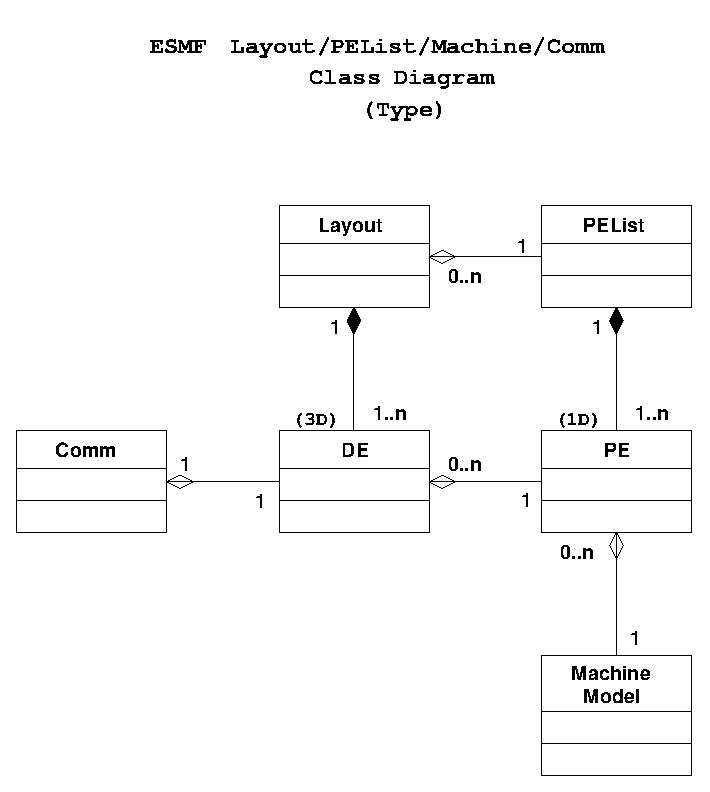
\includegraphics{CommMemClass.EPS}

Figure 1.  ESMF CommMem Class Diagram

\end{center}

\begin{center}
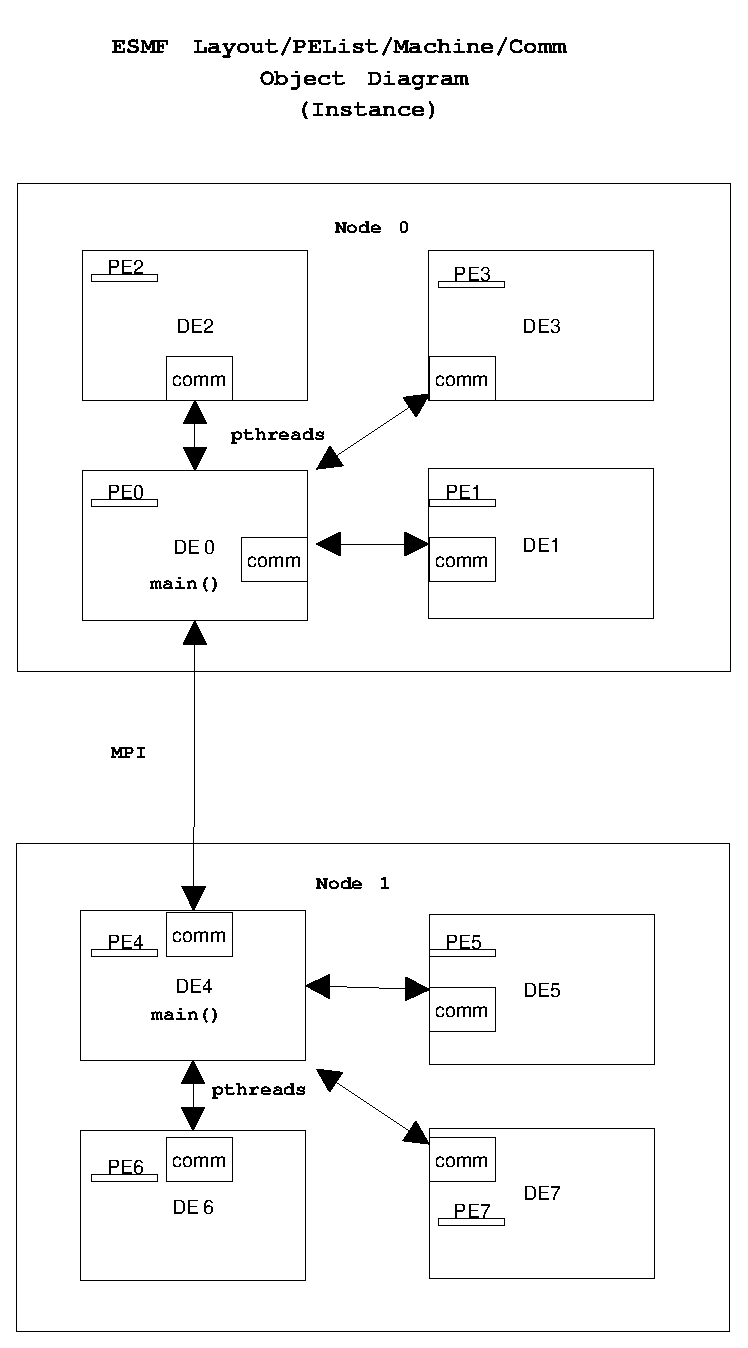
\includegraphics{CommMemObject.EPS}

Figure 2.  ESMF CommMem Example Object Diagram

\end{center}

\begin{center}
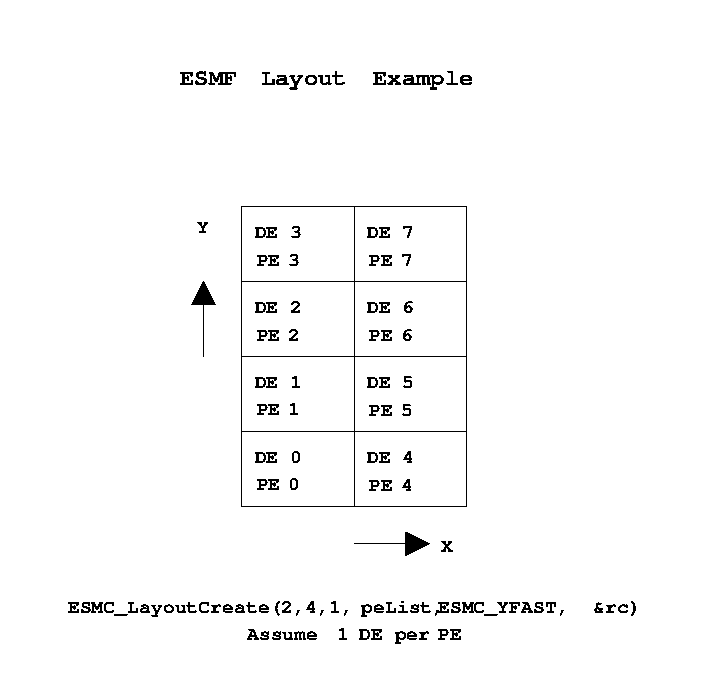
\includegraphics{DELayout.EPS}

Figure 3.  ESMF DELayout Example Object Diagram

\end{center}



\section{Global Parameters and Definitions}

% $Id: CommMem_param.tex,v 1.1 2002/12/10 03:08:26 eschwab Exp $

\begin{verbatim}
// shared memory local buffer for intra-node pthreads communications
int *lbuf = 0;

// shared memory global receive buffer for inter-node MPI communications
int *gbuf = 0;
\end{verbatim}



\section{Machine Class Design}

\subsection{Description}

% $Id: ESMC_Machine_desc.tex,v 1.1 2003/09/19 17:00:02 cdeluca Exp $

The Machine class encapsulates the required machine model information and
behavior.



\subsection{Design}

% $Id: ESMC_Machine_design.tex,v 1.1 2002/12/10 03:08:26 eschwab Exp $

The Machine class is designed to isolate and encapsulate system-dependent
information and functions other than for communication (see Comm class).
It provides an API to retrieve information such as the number of nodes,
number CPUs per node, IDs of particular hardware elements (PEs, nodes),
whether the machine provides MPI, pthreads and other communication services,
and various machine performance parameters such as bandwidths, latencies,
cache sizes, and FLOPS.



\subsubsection{Class Definition}

% $Id: ESMC_Machine_def.tex,v 1.1 2002/12/10 03:08:26 eschwab Exp $

\begin{verbatim}
 // class definition type
 class ESMC_Machine : public ESMC_Base {    // inherits from ESMC_Base class

   private:
 //  < insert class members here >  corresponds to type ESMF_Machine members
 //                                 in F90 modules
     int numNodes;         // number of nodes in machine or domain
     int numCPUs;          // number of CPUs in machine or domain
     int numCPUsperNode;   // number of CPUs per Node
     bool hasMPI;          // machine has MPI 1.2
     bool hasOpenMP;       // machine has OpenMP 1.0
     bool hasShmem;        // machine has Shmem
     bool hasPthreads;     // machine has pthreads
     int shMemLatency;     // latency of shared memory (microsec)
     int shMemBandwidth;   // bandwidth of shared memory (MB/s)
     int distMemLatency;   // latency of distributed memory (microsec)
     int distMemBandwidth; // bandwidth of distributed memory (MB/s)
\end{verbatim}



\subsubsection{Restrictions}

%\input{ESMC_Machine_rest}


\section{Machine Class F90 Interface}

\subsection{Use and Examples}

%\input{ESMC_Machine_fex}


\subsection{Parameters and Definitions}

%\input{ESMC_Machine_fparam}


%\subsection{Class API}

%\input{ESMC_Machine_fapi}


\section{Machine Class C++ Interface}

\subsection{Use and Examples}

% $Id: ESMC_Machine_ccex.tex,v 1.1 2003/09/19 17:00:02 cdeluca Exp $

See the example program on SourceForge under

esmf/src/Infrastructure/CommMem/examples/CMKex.C



\subsection{Parameters and Definitions}

%\input{ESMC_Machine_ccparam}


%\subsection{Class API}

%                **** IMPORTANT NOTICE *****
% This LaTeX file has been automatically produced by ProTeX v. 1.1
% Any changes made to this file will likely be lost next time
% this file is regenerated from its source. Send questions 
% to Arlindo da Silva, dasilva@gsfc.nasa.gov
 
\parskip        0pt
\parindent      0pt
\baselineskip  11pt
 
%--------------------- SHORT-HAND MACROS ----------------------
\def\bv{\begin{verbatim}}
\def\ev{\end{verbatim}}
\def\be{\begin{equation}}
\def\ee{\end{equation}}
\def\bea{\begin{eqnarray}}
\def\eea{\end{eqnarray}}
\def\bi{\begin{itemize}}
\def\ei{\end{itemize}}
\def\bn{\begin{enumerate}}
\def\en{\end{enumerate}}
\def\bd{\begin{description}}
\def\ed{\end{description}}
\def\({\left (}
\def\){\right )}
\def\[{\left [}
\def\]{\right ]}
\def\<{\left  \langle}
\def\>{\right \rangle}
\def\cI{{\cal I}}
\def\diag{\mathop{\rm diag}}
\def\tr{\mathop{\rm tr}}
%-------------------------------------------------------------

\markboth{Left}{Source File: ESMC\_Machine.h,  Date: Mon Dec  9 19:56:32 MST 2002
}

 
%/////////////////////////////////////////////////////////////
\subsection{C++:  Class Interface ESMC\_Machine - encapsulates platform capabilites and dependencies (Source File: ESMC\_Machine.h)}


  
  
   The code in this file defines the C++ Machine members and declares method 
   signatures (prototypes).  The companion file ESMC\_Machine.C contains
   the definitions (full code bodies) for the Machine methods.
  
   
  
  -----------------------------------------------------------------------------
   
\bigskip{\em USES:}
\begin{verbatim}  #include <ESMC_Base.h>  // all classes inherit from the ESMC Base class.
  //#include <ESMC_XXX.h>   // other dependent classes (subclasses, aggregates,
                         // composites, associates, friends)
 \end{verbatim}{\sf PUBLIC TYPES:}
\begin{verbatim}   class ESMC_MachineConfig;
  class ESMC_Machine;
 \end{verbatim}{\sf PRIVATE TYPES:}
\begin{verbatim} 
  // class configuration type
   class ESMC_MachineConfig {
     private:
  //   < insert resource items here >
   };
 
  // class definition type
  class ESMC_Machine : public ESMC_Base {    // inherits from ESMC_Base class
 
    private:
  //  < insert class members here >  corresponds to type ESMF_Machine members
  //                                 in F90 modules
      int numNodes;         // number of nodes in machine or domain
      int numCPUs;          // number of CPUs in machine or domain
      int numCPUsperNode;   // number of CPUs per Node
      bool hasMPI;          // machine has MPI 1.2
      bool hasOpenMP;       // machine has OpenMP 1.0
      bool hasShmem;        // machine has Shmem
      bool hasPthreads;     // machine has pthreads
      int shMemLatency;     // latency of shared memory (microsec)
      int shMemBandwidth;   // bandwidth of shared memory (MB/s)
      int distMemLatency;   // latency of distributed memory (microsec)
      int distMemBandwidth; // bandwidth of distributed memory (MB/s)
 \end{verbatim}{\sf PUBLIC MEMBER FUNCTIONS:}
\begin{verbatim}    public:
 
  // the following method applies to a shallow class
     int ESMC_MachineInit(int nodes, int cpus, int cpuspernode,
                          bool hasmpi, bool hasopenmp, bool hasshmem,
                          int shmemlat, int shmemband,
                          int distmemlat, int distmemband);
 
  // optional configuration methods
      int ESMC_MachineGetConfig(ESMC_MachineConfig *config) const;
      int ESMC_MachineSetConfig(const ESMC_MachineConfig *config);
 
  // accessor methods for class members
       int ESMC_MachineGetNumNodes(int *nodes) const;
       int ESMC_MachineSetNumNodes(int nodes);
       int ESMC_MachineGetNumCPUs(int *cpu) const;
       int ESMC_MachineSetNumCPUs(int cpu);
       int ESMC_MachineGetNumCPUsperNode(int *cpuspernode) const;
       int ESMC_MachineSetNumCPUsperNode(int cpuspernode);
 
       bool ESMC_MachineHasMPI(void);
       bool ESMC_MachineHasOpenMP(void);
       bool ESMC_MachineHasShmem(void);
       bool ESMC_MachineHasPthreads(void);
       int ESMC_MachineSetHasMPI(bool hasit);
       int ESMC_MachineSetOpenMP(bool hasit);
       int ESMC_MachineSetShmem(bool hasit);
       int ESMC_MachineSetPthreads(bool hasit);
 
       int ESMC_MachineGetshMemLatency(int *lat) const;
       int ESMC_MachineSetshMemLatency(int lat);
       int ESMC_MachineGetshMemBandwidth(int *bandw) const;
       int ESMC_MachineSetshMemBandwidth(int bandw);
       int ESMC_MachineGetdistMemLatency(int *lat) const;
       int ESMC_MachineSetdistMemLatency(int lat);
       int ESMC_MachineGetdistMemBandwidth(int *bandw) const;
       int ESMC_MachineSetdistMemBandwidth(int bandw);
     
  // required methods inherited and overridden from the ESMC_Base class
     int ESMC_MachineValidate(void) const;
     int ESMC_MachinePrint(void) const;
 
  // native C++ constructors/destructors
 	ESMC_Machine(void);
 	~ESMC_Machine(void);
   
  // < declare the rest of the public interface methods here >
 
   // get cpu id
   int ESMC_MachineGetCpuID(int *cpuid) const;
 
   // get node id
   int ESMC_MachineGetNodeID(int *nodeid) const;
 
   // get max cpus on a node
   int ESMC_MachineGetNodeCpuMax(int *maxcpus) const;
   \end{verbatim}{\sf PRIVATE MEMBER FUNCTIONS:}
\begin{verbatim}   private: 
  // < declare private interface methods here >\end{verbatim}

%...............................................................

%                **** IMPORTANT NOTICE *****
% This LaTeX file has been automatically produced by ProTeX v. 1.1
% Any changes made to this file will likely be lost next time
% this file is regenerated from its source. Send questions 
% to Arlindo da Silva, dasilva@gsfc.nasa.gov
 
\parskip        0pt
\parindent      0pt
\baselineskip  11pt
 
%--------------------- SHORT-HAND MACROS ----------------------
\def\bv{\begin{verbatim}}
\def\ev{\end{verbatim}}
\def\be{\begin{equation}}
\def\ee{\end{equation}}
\def\bea{\begin{eqnarray}}
\def\eea{\end{eqnarray}}
\def\bi{\begin{itemize}}
\def\ei{\end{itemize}}
\def\bn{\begin{enumerate}}
\def\en{\end{enumerate}}
\def\bd{\begin{description}}
\def\ed{\end{description}}
\def\({\left (}
\def\){\right )}
\def\[{\left [}
\def\]{\right ]}
\def\<{\left  \langle}
\def\>{\right \rangle}
\def\cI{{\cal I}}
\def\diag{\mathop{\rm diag}}
\def\tr{\mathop{\rm tr}}
%-------------------------------------------------------------

\markboth{Left}{Source File: ESMC\_Machine.C,  Date: Mon Dec  9 19:56:32 MST 2002
}

 
%/////////////////////////////////////////////////////////////
\subsubsection{ESMC\_MachineInit - initializes a Machine object}


  
\bigskip{\sf INTERFACE:}
\begin{verbatim}       int ESMC_Machine::ESMC_MachineInit(\end{verbatim}{\em RETURN VALUE:}
\begin{verbatim}      int error return code\end{verbatim}{\em ARGUMENTS:}
\begin{verbatim}       int nodes,          // in - number of nodes in machine or domain
       int cpus,           // in - number of cpus in machine or domain
       int cpuspernode,    // in - number of cpus per node in machine
       bool hasmpi,        // in - machine supports MPI 1.2
       bool hasopenmp,     // in - machine supports OpenMP 1.0
       bool hasshmem,      // in - machine supports Shmem
       int shmemlat,       // in - shared memory latency
       int shmemband,      // in - shared memory bandwidth
       int distmemlat,     // in - distributed memory latency
       int distmemband) {  // in - distributed memory bandwidth
       \end{verbatim}
{\sf DESCRIPTION:\\ }


        ESMF routine which only initializes Machine values; it does not
        allocate any resources. 
   
%/////////////////////////////////////////////////////////////
 
\mbox{}\hrulefill\ 
 
\subsubsection{ESMC\_MachineGetConfig - get configuration info from a Machine}


  
\bigskip{\sf INTERFACE:}
\begin{verbatim}       int ESMC_Machine::ESMC_MachineGetConfig(\end{verbatim}{\em RETURN VALUE:}
\begin{verbatim}      int error return code\end{verbatim}{\em ARGUMENTS:}
\begin{verbatim}       ESMC_MachineConfig *config) const {  // out - resources\end{verbatim}
{\sf DESCRIPTION:\\ }


      Returns the set of resources the Machine object was configured with.
   
%/////////////////////////////////////////////////////////////
 
\mbox{}\hrulefill\ 
 
\subsubsection{ESMC\_MachineSetConfig - set configuration info for a Machine}


  
\bigskip{\sf INTERFACE:}
\begin{verbatim}       int ESMC_Machine::ESMC_MachineSetConfig(\end{verbatim}{\em RETURN VALUE:}
\begin{verbatim}      int error return code\end{verbatim}{\em ARGUMENTS:}
\begin{verbatim}       const ESMC_MachineConfig *config) {     // in - resources\end{verbatim}
{\sf DESCRIPTION:\\ }


      Configures the Machine object with set of resources given.
   
%/////////////////////////////////////////////////////////////
 
\mbox{}\hrulefill\ 
 
\subsubsection{ESMC\_MachineGet<Value> - get <Value> for a Machine}


  
\bigskip{\sf INTERFACE:}
\begin{verbatim}       int ESMC_Machine::ESMC_MachineGet<Value>(\end{verbatim}{\em RETURN VALUE:}
\begin{verbatim}      int error return code\end{verbatim}{\em ARGUMENTS:}
\begin{verbatim}       <value type> *value) const {     // out - value\end{verbatim}
{\sf DESCRIPTION:\\ }


       Returns the value of Machine member <Value>.
       Can be multiple routines, one per value
   
%/////////////////////////////////////////////////////////////
 
\mbox{}\hrulefill\ 
 
\subsubsection{ESMC\_MachineSet<Value> - set <Value> for a Machine}


  
\bigskip{\sf INTERFACE:}
\begin{verbatim}       int ESMC_Machine::ESMC_MachineSet<Value>(\end{verbatim}{\em RETURN VALUE:}
\begin{verbatim}      int error return code\end{verbatim}{\em ARGUMENTS:}
\begin{verbatim}       <value type> value) {     // in - value\end{verbatim}
{\sf DESCRIPTION:\\ }


       Sets the Machine member <Value> with the given value.
       Can be multiple routines, one per value
   
%/////////////////////////////////////////////////////////////
 
\mbox{}\hrulefill\ 
 
\subsubsection{ESMC\_MachineValidate - internal consistency check for a Machine}


  
\bigskip{\sf INTERFACE:}
\begin{verbatim}       int ESMC_Machine::ESMC_MachineValidate(\end{verbatim}{\em RETURN VALUE:}
\begin{verbatim}      int error return code\end{verbatim}{\em ARGUMENTS:}
\begin{verbatim}       void) const {    // in - validate options\end{verbatim}
{\sf DESCRIPTION:\\ }


        Validates that a Machine is internally consistent.
        Returns error code if problems are found.  ESMC\_Base class method.
   
%/////////////////////////////////////////////////////////////
 
\mbox{}\hrulefill\ 
 
\subsubsection{ESMC\_MachinePrint - print contents of a Machine}


  
\bigskip{\sf INTERFACE:}
\begin{verbatim}       int ESMC_Machine::ESMC_MachinePrint(\end{verbatim}{\em RETURN VALUE:}
\begin{verbatim}      int error return code\end{verbatim}{\em ARGUMENTS:}
\begin{verbatim}       void) const {     //  in - print options\end{verbatim}
{\sf DESCRIPTION:\\ }


        Print information about a Machine.  The options control the
        type of information and level of detail.  ESMC\_Base class method.
   
%/////////////////////////////////////////////////////////////
 
\mbox{}\hrulefill\ 
 
\subsubsection{ESMC\_Machine - native C++ constructor}


  
\bigskip{\sf INTERFACE:}
\begin{verbatim}       ESMC_Machine::ESMC_Machine(\end{verbatim}{\em RETURN VALUE:}
\begin{verbatim}      none\end{verbatim}{\em ARGUMENTS:}
\begin{verbatim}       void) {  // in\end{verbatim}
{\sf DESCRIPTION:\\ }


        Calls standard ESMF deep or shallow methods for initialization
        with default or passed-in values
   
%/////////////////////////////////////////////////////////////
 
\mbox{}\hrulefill\ 
 
\subsubsection{~ESMC\_Machine - native C++ destructor}


  
\bigskip{\sf INTERFACE:}
\begin{verbatim}       ESMC_Machine::~ESMC_Machine(void) {\end{verbatim}{\em RETURN VALUE:}
\begin{verbatim}      none\end{verbatim}{\em ARGUMENTS:}
\begin{verbatim}      none\end{verbatim}
{\sf DESCRIPTION:\\ }


        Calls standard ESMF deep or shallow methods for destruction
   
%/////////////////////////////////////////////////////////////
 
\mbox{}\hrulefill\ 
 
\subsubsection{ESMC\_MachineGetCpuID - get the machine-specific Cpu ID}


  
\bigskip{\sf INTERFACE:}
\begin{verbatim}       int ESMC_Machine::ESMC_MachineGetCpuID(\end{verbatim}{\em RETURN VALUE:}
\begin{verbatim}      int error return code\end{verbatim}{\em ARGUMENTS:}
\begin{verbatim}       int *cpuid) const {     // out - Cpu ID\end{verbatim}
{\sf DESCRIPTION:\\ }


       Returns the Cpu ID of the calling process/thread
   
%/////////////////////////////////////////////////////////////
 
\mbox{}\hrulefill\ 
 
\subsubsection{ESMC\_MachineGetNodeID - get the machine-specific Node ID}


  
\bigskip{\sf INTERFACE:}
\begin{verbatim}       int ESMC_Machine::ESMC_MachineGetNodeID(\end{verbatim}{\em RETURN VALUE:}
\begin{verbatim}      int error return code\end{verbatim}{\em ARGUMENTS:}
\begin{verbatim}       int *nodeid) const {     // out - Node ID\end{verbatim}
{\sf DESCRIPTION:\\ }


       Returns the Node ID of the calling process/thread
   
%/////////////////////////////////////////////////////////////
 
\mbox{}\hrulefill\ 
 
\subsubsection{ESMC\_MachineGetNodeCpuMax - get the max Cpus per Node}


  
\bigskip{\sf INTERFACE:}
\begin{verbatim}       int ESMC_Machine::ESMC_MachineGetNodeCpuMax(\end{verbatim}{\em RETURN VALUE:}
\begin{verbatim}      int error return code\end{verbatim}{\em ARGUMENTS:}
\begin{verbatim}       int *maxcpus) const {     // out - max cpus per node\end{verbatim}
{\sf DESCRIPTION:\\ }


       Returns the maximum number of cpus per node
  
%...............................................................



\section{PE Class Design}

\subsection{Description}

% $Id: ESMC_PE_desc.tex,v 1.1 2002/12/10 03:08:26 eschwab Exp $

The PE class encapsulates the required processor information and
behavior.



\subsection{Design}

% $Id: ESMC_PE_design.tex,v 1.1 2003/09/19 17:00:02 cdeluca Exp $

The PE class encapsulates machine dependent identifying information about
a processing element, such as cpu ID and node ID.  A machine-indendent ESMF ID
is also assigned.  A PE is instantiated within a DE upon startup and self-
discovers its cpu and node IDs.  This information from all DE's is then
gathered to form the PE list.



\subsubsection{Class Definition}

% $Id: ESMC_PE_def.tex,v 1.1 2003/09/19 17:00:02 cdeluca Exp $

\begin{verbatim}
 // class declaration type
 class ESMC_PE : public ESMC_Base {    // inherits from ESMC_Base class

   private:
 //  < insert class members here >  corresponds to type ESMF_PE members
 //                                 in F90 modules
    int esmfID;    // ESMF assigned ID
    int cpuID;     // Hardware assigned processor ID
    int nodeID;    // hardware assigned associated node ID
    static int peCount;  // number of PEs instantiated

    ESMC_Machine *machine;  // interface to specific platform
\end{verbatim}



\subsubsection{Restrictions}

%\input{ESMC_PE_rest}


\section{PE Class F90 Interface}

\subsection{Use and Examples}

%\input{ESMC_PE_fex}


\subsection{Parameters and Definitions}

%\input{ESMC_PE_fparam}


%\subsection{Class API}

%\input{ESMC_PE_fapi}


\section{PE Class C++ Interface}

\subsection{Use and Examples}

% $Id: ESMC_PE_ccex.tex,v 1.1 2002/12/10 03:08:26 eschwab Exp $

See the example program on SourceForge under

esmf/src/Infrastructure/CommMem/examples/CMKex.C



\subsection{Parameters and Definitions}

%\input{ESMC_PE_ccparam}


%\subsection{Class API}

%                **** IMPORTANT NOTICE *****
% This LaTeX file has been automatically produced by ProTeX v. 1.1
% Any changes made to this file will likely be lost next time
% this file is regenerated from its source. Send questions 
% to Arlindo da Silva, dasilva@gsfc.nasa.gov
 
\parskip        0pt
\parindent      0pt
\baselineskip  11pt
 
%--------------------- SHORT-HAND MACROS ----------------------
\def\bv{\begin{verbatim}}
\def\ev{\end{verbatim}}
\def\be{\begin{equation}}
\def\ee{\end{equation}}
\def\bea{\begin{eqnarray}}
\def\eea{\end{eqnarray}}
\def\bi{\begin{itemize}}
\def\ei{\end{itemize}}
\def\bn{\begin{enumerate}}
\def\en{\end{enumerate}}
\def\bd{\begin{description}}
\def\ed{\end{description}}
\def\({\left (}
\def\){\right )}
\def\[{\left [}
\def\]{\right ]}
\def\<{\left  \langle}
\def\>{\right \rangle}
\def\cI{{\cal I}}
\def\diag{\mathop{\rm diag}}
\def\tr{\mathop{\rm tr}}
%-------------------------------------------------------------

\markboth{Left}{Source File: ESMC\_PE.h,  Date: Mon Dec  9 19:56:32 MST 2002
}

 
%/////////////////////////////////////////////////////////////
\subsection{C++:  Class Interface ESMC\_PE - one line general statement about this class (Source File: ESMC\_PE.h)}


  
  
   The code in this file defines the C++ PE members and declares method 
   signatures (prototypes).  The companion file ESMC\_PE.C contains
   the definitions (full code bodies) for the PE methods.
  
   < insert a paragraph or two explaining what you'll find in this file >
  
  -----------------------------------------------------------------------------
   
\bigskip{\em USES:}
\begin{verbatim}  #include <ESMC_Base.h>  // all classes inherit from the ESMC Base class.
  #include <ESMC_Machine.h>  
  //#include <ESMC_XXX.h>   // other dependent classes (subclasses, aggregates,
                         // composites, associates, friends)
 \end{verbatim}{\sf PUBLIC TYPES:}
\begin{verbatim}   class ESMC_PEConfig;
  class ESMC_PE;
 \end{verbatim}{\sf PRIVATE TYPES:}
\begin{verbatim} 
  // class configuration type
   class ESMC_PEConfig {
     private:
  //   < insert resource items here >
   };
 
  // class declaration type
  class ESMC_PE : public ESMC_Base {    // inherits from ESMC_Base class
 
    private:
  //  < insert class members here >  corresponds to type ESMF_PE members
  //                                 in F90 modules
     int esmfID;    // ESMF assigned ID
     int cpuID;     // Hardware assigned processor ID
     int nodeID;    // hardware assigned associated node ID
     static int peCount;  // number of PEs instantiated
 
     ESMC_Machine *machine;  // interface to specific platform
     // neighbor connections ?  see ESMC_Layout.h
 \end{verbatim}{\sf PUBLIC MEMBER FUNCTIONS:}
\begin{verbatim}   public:
  // the following method applies to a shallow class
     int ESMC_PEInit(void);
     int ESMC_PEInit(int esmfid, int cpuid, int nodeid);
 
  // optional configuration methods
      int ESMC_PEGetConfig(ESMC_PEConfig *config) const;
      int ESMC_PESetConfig(const ESMC_PEConfig *config);
 
  // accessor methods for class members
     int ESMC_PEGetEsmfID(int *id) const;
     int ESMC_PESetEsmfID(int  id);
 
     int ESMC_PEGetCpuID(int *id) const;
     int ESMC_PESetCpuID(int  id);
 
     int ESMC_PEGetNodeID(int *id) const;
     int ESMC_PESetNodeID(int  id);
     
  // required methods inherited and overridden from the ESMC_Base class
     int ESMC_PEValidate(void) const;
     int ESMC_PEPrint(void) const;
 
  // native C++ constructors/destructors
 	ESMC_PE(void);
 	~ESMC_PE(void);
   
  // < declare the rest of the public interface methods here >
 
     // friend int ESMC_PEListPECompare(const void *pe1, const void *pe2);
     // friend class ESMC_PEList;  // TODO: ?? implement in ESMC_PEList
   \end{verbatim}{\sf PRIVATE MEMBER FUNCTIONS:}
\begin{verbatim}   private: 
  // < declare private interface methods here >\end{verbatim}

%...............................................................

%                **** IMPORTANT NOTICE *****
% This LaTeX file has been automatically produced by ProTeX v. 1.1
% Any changes made to this file will likely be lost next time
% this file is regenerated from its source. Send questions 
% to Arlindo da Silva, dasilva@gsfc.nasa.gov
 
\parskip        0pt
\parindent      0pt
\baselineskip  11pt
 
%--------------------- SHORT-HAND MACROS ----------------------
\def\bv{\begin{verbatim}}
\def\ev{\end{verbatim}}
\def\be{\begin{equation}}
\def\ee{\end{equation}}
\def\bea{\begin{eqnarray}}
\def\eea{\end{eqnarray}}
\def\bi{\begin{itemize}}
\def\ei{\end{itemize}}
\def\bn{\begin{enumerate}}
\def\en{\end{enumerate}}
\def\bd{\begin{description}}
\def\ed{\end{description}}
\def\({\left (}
\def\){\right )}
\def\[{\left [}
\def\]{\right ]}
\def\<{\left  \langle}
\def\>{\right \rangle}
\def\cI{{\cal I}}
\def\diag{\mathop{\rm diag}}
\def\tr{\mathop{\rm tr}}
%-------------------------------------------------------------

\markboth{Left}{Source File: ESMC\_PE.C,  Date: Mon Dec  9 19:56:32 MST 2002
}

 
%/////////////////////////////////////////////////////////////
\subsubsection{ESMC\_PEInit - initializes a PE object}


  
\bigskip{\sf INTERFACE:}
\begin{verbatim}       int ESMC_PE::ESMC_PEInit(\end{verbatim}{\em RETURN VALUE:}
\begin{verbatim}      int error return code\end{verbatim}{\em ARGUMENTS:}
\begin{verbatim}       void) {         //\end{verbatim}
{\sf DESCRIPTION:\\ }


        ESMF routine which only initializes PE values; it does not
        allocate any resources.
   
%/////////////////////////////////////////////////////////////
 
\mbox{}\hrulefill\ 
 
\subsubsection{ESMC\_PEInit - initializes a PE object}


  
\bigskip{\sf INTERFACE:}
\begin{verbatim}       int ESMC_PE::ESMC_PEInit(\end{verbatim}{\em RETURN VALUE:}
\begin{verbatim}      int error return code\end{verbatim}{\em ARGUMENTS:}
\begin{verbatim}       int esmfid,           // in
       int cpuid,            // in
       int nodeid) {         // in\end{verbatim}
{\sf DESCRIPTION:\\ }


        ESMF routine which only initializes PE values; it does not
        allocate any resources.
   
%/////////////////////////////////////////////////////////////
 
\mbox{}\hrulefill\ 
 
\subsubsection{ESMC\_PEGetConfig - get configuration info from a PE}


  
\bigskip{\sf INTERFACE:}
\begin{verbatim}       int ESMC_PE::ESMC_PEGetConfig(\end{verbatim}{\em RETURN VALUE:}
\begin{verbatim}      int error return code\end{verbatim}{\em ARGUMENTS:}
\begin{verbatim}       ESMC_PEConfig *config) const {  // out - resources\end{verbatim}
{\sf DESCRIPTION:\\ }


      Returns the set of resources the PE object was configured with.
   
%/////////////////////////////////////////////////////////////
 
\mbox{}\hrulefill\ 
 
\subsubsection{ESMC\_PESetConfig - set configuration info for a PE}


  
\bigskip{\sf INTERFACE:}
\begin{verbatim}       int ESMC_PE::ESMC_PESetConfig(\end{verbatim}{\em RETURN VALUE:}
\begin{verbatim}      int error return code\end{verbatim}{\em ARGUMENTS:}
\begin{verbatim}       const ESMC_PEConfig *config) {     // in - resources\end{verbatim}
{\sf DESCRIPTION:\\ }


      Configures the PE object with set of resources given.
   
%/////////////////////////////////////////////////////////////
 
\mbox{}\hrulefill\ 
 
\subsubsection{ESMC\_PEGetEsmfID - get esmfID for a PE}


  
\bigskip{\sf INTERFACE:}
\begin{verbatim}       int ESMC_PE::ESMC_PEGetEsmfID(\end{verbatim}{\em RETURN VALUE:}
\begin{verbatim}      int error return code\end{verbatim}{\em ARGUMENTS:}
\begin{verbatim}       int *esmfid) const {     // out - esmfid\end{verbatim}
{\sf DESCRIPTION:\\ }


       Returns the value of PE member esmfID
   
%/////////////////////////////////////////////////////////////
 
\mbox{}\hrulefill\ 
 
\subsubsection{ESMC\_PESetEsmfID - set esmfID for a PE}


  
\bigskip{\sf INTERFACE:}
\begin{verbatim}       int ESMC_PE::ESMC_PESetEsmfID(\end{verbatim}{\em RETURN VALUE:}
\begin{verbatim}      int error return code\end{verbatim}{\em ARGUMENTS:}
\begin{verbatim}       int esmfid) {     // in - value\end{verbatim}
{\sf DESCRIPTION:\\ }


       Sets the PE member esmfID with the given value.
   
%/////////////////////////////////////////////////////////////
 
\mbox{}\hrulefill\ 
 
\subsubsection{ESMC\_PEGetCpuID - get cpuID for a PE}


  
\bigskip{\sf INTERFACE:}
\begin{verbatim}       int ESMC_PE::ESMC_PEGetCpuID(\end{verbatim}{\em RETURN VALUE:}
\begin{verbatim}      int error return code\end{verbatim}{\em ARGUMENTS:}
\begin{verbatim}       int *cpuid) const {     // out - cpuid\end{verbatim}
{\sf DESCRIPTION:\\ }


       Returns the value of PE member cpuID
   
%/////////////////////////////////////////////////////////////
 
\mbox{}\hrulefill\ 
 
\subsubsection{ESMC\_PESetCpuID - set cpuID for a PE}


  
\bigskip{\sf INTERFACE:}
\begin{verbatim}       int ESMC_PE::ESMC_PESetCpuID(\end{verbatim}{\em RETURN VALUE:}
\begin{verbatim}      int error return code\end{verbatim}{\em ARGUMENTS:}
\begin{verbatim}       int cpuid) {     // in - value\end{verbatim}
{\sf DESCRIPTION:\\ }


       Sets the PE member cpuID with the given value.
   
%/////////////////////////////////////////////////////////////
 
\mbox{}\hrulefill\ 
 
\subsubsection{ESMC\_PEGetNodeID - get nodeID for a PE}


  
\bigskip{\sf INTERFACE:}
\begin{verbatim}       int ESMC_PE::ESMC_PEGetNodeID(\end{verbatim}{\em RETURN VALUE:}
\begin{verbatim}      long error return code\end{verbatim}{\em ARGUMENTS:}
\begin{verbatim}       int *nodeid) const {     // out - nodeid\end{verbatim}
{\sf DESCRIPTION:\\ }


       Returns the value of PE member nodeID
   
%/////////////////////////////////////////////////////////////
 
\mbox{}\hrulefill\ 
 
\subsubsection{ESMC\_PESetNodeID - set nodeID for a PE}


  
\bigskip{\sf INTERFACE:}
\begin{verbatim}       int ESMC_PE::ESMC_PESetNodeID(\end{verbatim}{\em RETURN VALUE:}
\begin{verbatim}      int error return code\end{verbatim}{\em ARGUMENTS:}
\begin{verbatim}       int nodeid) {     // in - value\end{verbatim}
{\sf DESCRIPTION:\\ }


       Sets the PE member nodeID with the given value.
   
%/////////////////////////////////////////////////////////////
 
\mbox{}\hrulefill\ 
 
\subsubsection{ESMC\_PEValidate - internal consistency check for a PE}


  
\bigskip{\sf INTERFACE:}
\begin{verbatim}       int ESMC_PE::ESMC_PEValidate(\end{verbatim}{\em RETURN VALUE:}
\begin{verbatim}      int error return code\end{verbatim}{\em ARGUMENTS:}
\begin{verbatim}       void) const {    // in - validate options\end{verbatim}
{\sf DESCRIPTION:\\ }


        Validates that a PE is internally consistent.
        Returns error code if problems are found.  ESMC\_Base class method.
   
%/////////////////////////////////////////////////////////////
 
\mbox{}\hrulefill\ 
 
\subsubsection{ESMC\_PEPrint - print contents of a PE}


  
\bigskip{\sf INTERFACE:}
\begin{verbatim}       int ESMC_PE::ESMC_PEPrint(\end{verbatim}{\em RETURN VALUE:}
\begin{verbatim}      int error return code\end{verbatim}{\em ARGUMENTS:}
\begin{verbatim}       void) const {     //  in - print options\end{verbatim}
{\sf DESCRIPTION:\\ }


        Print information about a PE.  The options control the
        type of information and level of detail.  ESMC\_Base class method.
   
%/////////////////////////////////////////////////////////////
 
\mbox{}\hrulefill\ 
 
\subsubsection{ESMC\_PE - native C++ constructor}


  
\bigskip{\sf INTERFACE:}
\begin{verbatim}       ESMC_PE::ESMC_PE(\end{verbatim}{\em RETURN VALUE:}
\begin{verbatim}      none\end{verbatim}{\em ARGUMENTS:}
\begin{verbatim}       void) {\end{verbatim}
{\sf DESCRIPTION:\\ }


        Calls standard ESMF deep or shallow methods for initialization
        with default or passed-in values
   
%/////////////////////////////////////////////////////////////
 
\mbox{}\hrulefill\ 
 
\subsubsection{~ESMC\_PE - native C++ destructor}


  
\bigskip{\sf INTERFACE:}
\begin{verbatim}       ESMC_PE::~ESMC_PE(void) {\end{verbatim}{\em RETURN VALUE:}
\begin{verbatim}      none\end{verbatim}{\em ARGUMENTS:}
\begin{verbatim}      none\end{verbatim}
{\sf DESCRIPTION:\\ }


        Calls standard ESMF deep or shallow methods for destruction
  
%...............................................................



\section{DE Class Design}

\subsection{Description}

% $Id: ESMC_DE_desc.tex,v 1.1 2002/12/10 03:08:26 eschwab Exp $

The DE class encapsulates distributed element (processes and threads)
information and behavior.



\subsection{Design}

% $Id: ESMC_DE_design.tex,v 1.2 2003/03/10 03:22:57 cdeluca Exp $

The DE class encapsulates a process or thread's identifying information.  This
includes whether the DE is a process or a thread as well as a system-dependent
process ID or thread ID, respectively.  A system-independent ESMF ID is also
assigned to the DE.  In addition, the PE on which the DE is running is
captured.  Upon system startup, a DE object is instantiated within each process
or thread.  The DE object self-discovers its ID information as well as its PE
assignment.  This is information is gathered across all DEs, and in
conjunction with the PE list, is used to create the DELayout.



\subsubsection{Class Definition}

% $Id: ESMC_DE_def.tex,v 1.1 2002/12/10 03:08:26 eschwab Exp $

\begin{verbatim}
 // class declaration type
 class ESMC_DE : public ESMC_Base {    // inherits from ESMC_Base class

   private:
 //  < insert class members here >  corresponds to type ESMF_DE members
 //                                 in F90 modules
     int esmfID;     // ESMF assigned ID
     int pID;        // processID (index)
     int tID;        // threadID (index)
     ESMC_DEType_e deType;  // process or thread
     bool process;   // true if DE is a process
     bool thread;    // true if DE is a thread
     ESMC_PE *PE;    // assigned PE from peList
\end{verbatim}



\subsubsection{Restrictions}

%\input{ESMC_DE_rest}


\section{DE Class F90 Interface}

\subsection{Use and Examples}

%\input{ESMC_DE_fex}


\subsection{Parameters and Definitions}

%\input{ESMC_DE_fparam}


%\subsection{Class API}

%\input{ESMC_DE_fapi}


\section{DE Class C++ Interface}

\subsection{Use and Examples}

% $Id: ESMC_DE_ccex.tex,v 1.1 2002/12/10 03:08:26 eschwab Exp $

See the example program on SourceForge under

esmf/src/Infrastructure/CommMem/examples/CMKex.C



\subsection{Parameters and Definitions}

%\input{ESMC_DE_ccparam}


%\subsection{Class API}

%                **** IMPORTANT NOTICE *****
% This LaTeX file has been automatically produced by ProTeX v. 1.1
% Any changes made to this file will likely be lost next time
% this file is regenerated from its source. Send questions 
% to Arlindo da Silva, dasilva@gsfc.nasa.gov
 
\parskip        0pt
\parindent      0pt
\baselineskip  11pt
 
%--------------------- SHORT-HAND MACROS ----------------------
\def\bv{\begin{verbatim}}
\def\ev{\end{verbatim}}
\def\be{\begin{equation}}
\def\ee{\end{equation}}
\def\bea{\begin{eqnarray}}
\def\eea{\end{eqnarray}}
\def\bi{\begin{itemize}}
\def\ei{\end{itemize}}
\def\bn{\begin{enumerate}}
\def\en{\end{enumerate}}
\def\bd{\begin{description}}
\def\ed{\end{description}}
\def\({\left (}
\def\){\right )}
\def\[{\left [}
\def\]{\right ]}
\def\<{\left  \langle}
\def\>{\right \rangle}
\def\cI{{\cal I}}
\def\diag{\mathop{\rm diag}}
\def\tr{\mathop{\rm tr}}
%-------------------------------------------------------------

\markboth{Left}{Source File: ESMC\_DE.h,  Date: Mon Dec  9 19:56:31 MST 2002
}

 
%/////////////////////////////////////////////////////////////
\subsection{C++:  Class Interface ESMC\_DE - Decomposition element (Source File: ESMC\_DE.h)}


  
  
   The code in this file defines the C++ DE members and declares method 
   signatures (prototypes).  The companion file ESMC\_DE.C contains
   the definitions (full code bodies) for the DE methods.
  
   ESMF abstraction of a process or thread
  
  -----------------------------------------------------------------------------
   
\bigskip{\em USES:}
\begin{verbatim}  #include <ESMC_Base.h>  // all classes inherit from the ESMC Base class.
  #include <ESMC_PE.h> 
  //#include <ESMC_XXX.h>   // other dependent classes (subclasses, aggregates,
                         // composites, associates, friends)
 
 enum ESMC_DEType_e {ESMC_PROCESS, ESMC_THREAD};
 \end{verbatim}{\sf PUBLIC TYPES:}
\begin{verbatim}   class ESMC_DEConfig;
  class ESMC_DE;
 \end{verbatim}{\sf PRIVATE TYPES:}
\begin{verbatim} 
  // class configuration type
   class ESMC_DEConfig {
     private:
  //   < insert resource items here >
   };
 
  // class declaration type
  class ESMC_DE : public ESMC_Base {    // inherits from ESMC_Base class
 
    private:
  //  < insert class members here >  corresponds to type ESMF_DE members
  //                                 in F90 modules
      int esmfID;     // ESMF assigned ID
      int pID;        // processID (index)
      int tID;        // threadID (index)
      ESMC_DEType_e deType;  // process or thread
      bool process;   // true if DE is a process
      bool thread;    // true if DE is a thread
      ESMC_PE *PE;    // assigned PE from peList
 \end{verbatim}{\sf PUBLIC MEMBER FUNCTIONS:}
\begin{verbatim}   public:
     int ESMC_DEInit(int esmfid, int pid, int tid, bool proc, bool thrd,
                     ESMC_PE *pe);
 
  // optional configuration methods
      int ESMC_DEGetConfig(ESMC_DEConfig *config) const;
      int ESMC_DESetConfig(const ESMC_DEConfig *config);
 
  // accessor methods for class members
      int ESMC_DEGet<Value>(<value type> *value) const;
      int ESMC_DESet<Value>(<value type>  value);
     int ESMC_DESetPE(ESMC_PE *pe);
     int ESMC_DESetESMFID(int esmfid);
     int ESMC_DEGetESMFID(int *esmfid) const;
     int ESMC_DEGetpID(int *pid) const;
     int ESMC_DEGetType(ESMC_DEType_e *detype) const;
     
  // required methods inherited and overridden from the ESMC_Base class
     int ESMC_DEValidate(void) const;
     int ESMC_DEPrint(void) const;
 
  // native C++ constructors/destructors
 	ESMC_DE(void);
 	ESMC_DE(ESMC_DEType_e detype);
 	~ESMC_DE(void);
   
  // < declare the rest of the public interface methods here >
 
     friend class ESMC_Comm;
     friend class ESMC_DELayout;
   \end{verbatim}{\sf PRIVATE MEMBER FUNCTIONS:}
\begin{verbatim}   private: 
  // < declare private interface methods here >\end{verbatim}

%...............................................................

%                **** IMPORTANT NOTICE *****
% This LaTeX file has been automatically produced by ProTeX v. 1.1
% Any changes made to this file will likely be lost next time
% this file is regenerated from its source. Send questions 
% to Arlindo da Silva, dasilva@gsfc.nasa.gov
 
\parskip        0pt
\parindent      0pt
\baselineskip  11pt
 
%--------------------- SHORT-HAND MACROS ----------------------
\def\bv{\begin{verbatim}}
\def\ev{\end{verbatim}}
\def\be{\begin{equation}}
\def\ee{\end{equation}}
\def\bea{\begin{eqnarray}}
\def\eea{\end{eqnarray}}
\def\bi{\begin{itemize}}
\def\ei{\end{itemize}}
\def\bn{\begin{enumerate}}
\def\en{\end{enumerate}}
\def\bd{\begin{description}}
\def\ed{\end{description}}
\def\({\left (}
\def\){\right )}
\def\[{\left [}
\def\]{\right ]}
\def\<{\left  \langle}
\def\>{\right \rangle}
\def\cI{{\cal I}}
\def\diag{\mathop{\rm diag}}
\def\tr{\mathop{\rm tr}}
%-------------------------------------------------------------

\markboth{Left}{Source File: ESMC\_DE.C,  Date: Mon Dec  9 19:56:32 MST 2002
}

 
%/////////////////////////////////////////////////////////////
\subsubsection{ESMC\_DEInit - initializes a DE object}


  
\bigskip{\sf INTERFACE:}
\begin{verbatim}       int ESMC_DE::ESMC_DEInit(\end{verbatim}{\em RETURN VALUE:}
\begin{verbatim}      int error return code\end{verbatim}{\em ARGUMENTS:}
\begin{verbatim}       int esmfid,                  // in - ESMF ID
       int pid,                     // in - platform process ID
       int tid,                     // in - platform thread ID
       bool proc,                   // in - true if DE is a process
       bool thrd,                   // in - true if DE is a thread
       ESMC_PE *pe) {               // in - assigned PE from peList\end{verbatim}
{\sf DESCRIPTION:\\ }


        ESMF routine which only initializes DE values; it does not
        allocate any resources.  Define for shallow classes only,
        for deep classes define and use routines Create/Destroy and
        Construct/Destruct.  Can be overloaded like ESMC\_DECreate.
   
%/////////////////////////////////////////////////////////////
 
\mbox{}\hrulefill\ 
 
\subsubsection{ESMC\_DEGetConfig - get configuration info from a DE}


  
\bigskip{\sf INTERFACE:}
\begin{verbatim}       int ESMC_DE::ESMC_DEGetConfig(\end{verbatim}{\em RETURN VALUE:}
\begin{verbatim}      int error return code\end{verbatim}{\em ARGUMENTS:}
\begin{verbatim}       ESMC_DEConfig *config) const {  // out - resources\end{verbatim}
{\sf DESCRIPTION:\\ }


      Returns the set of resources the DE object was configured with.
   
%/////////////////////////////////////////////////////////////
 
\mbox{}\hrulefill\ 
 
\subsubsection{ESMC\_DESetConfig - set configuration info for a DE}


  
\bigskip{\sf INTERFACE:}
\begin{verbatim}       int ESMC_DE::ESMC_DESetConfig(\end{verbatim}{\em RETURN VALUE:}
\begin{verbatim}      int error return code\end{verbatim}{\em ARGUMENTS:}
\begin{verbatim}       const ESMC_DEConfig *config) {     // in - resources\end{verbatim}
{\sf DESCRIPTION:\\ }


      Configures the DE object with set of resources given.
   
%/////////////////////////////////////////////////////////////
 
\mbox{}\hrulefill\ 
 
\subsubsection{ESMC\_DEGet<Value> - get <Value> for a DE}


  
\bigskip{\sf INTERFACE:}
\begin{verbatim}       int ESMC_DE::ESMC_DEGet<Value>(\end{verbatim}{\em RETURN VALUE:}
\begin{verbatim}      int error return code\end{verbatim}{\em ARGUMENTS:}
\begin{verbatim}       <value type> *value) const {     // out - value\end{verbatim}
{\sf DESCRIPTION:\\ }


       Returns the value of DE member <Value>.
       Can be multiple routines, one per value
   
%/////////////////////////////////////////////////////////////
 
\mbox{}\hrulefill\ 
 
\subsubsection{ESMC\_DESet<Value> - set <Value> for a DE}


  
\bigskip{\sf INTERFACE:}
\begin{verbatim}       int ESMC_DE::ESMC_DESet<Value>(\end{verbatim}{\em RETURN VALUE:}
\begin{verbatim}      int error return code\end{verbatim}{\em ARGUMENTS:}
\begin{verbatim}       <value type> value) {     // in - value\end{verbatim}
{\sf DESCRIPTION:\\ }


       Sets the DE member <Value> with the given value.
       Can be multiple routines, one per value
   
%/////////////////////////////////////////////////////////////
 
\mbox{}\hrulefill\ 
 
\subsubsection{ESMC\_DESetESMFID - set ESMF ID for this DE}


  
\bigskip{\sf INTERFACE:}
\begin{verbatim}       int ESMC_DE::ESMC_DESetESMFID(\end{verbatim}{\em RETURN VALUE:}
\begin{verbatim}      int error return code\end{verbatim}{\em ARGUMENTS:}
\begin{verbatim}       int esmfid) {     // in - ESMF ID\end{verbatim}
{\sf DESCRIPTION:\\ }


       Sets the ESMF ID for this DE to given value.
   
%/////////////////////////////////////////////////////////////
 
\mbox{}\hrulefill\ 
 
\subsubsection{ESMC\_DESetPE - assign PE to a DE}


  
\bigskip{\sf INTERFACE:}
\begin{verbatim}       int ESMC_DE::ESMC_DESetPE(\end{verbatim}{\em RETURN VALUE:}
\begin{verbatim}      int error return code\end{verbatim}{\em ARGUMENTS:}
\begin{verbatim}       ESMC_PE *pe) {     // in - PE\end{verbatim}
{\sf DESCRIPTION:\\ }


       Sets the DE member PE with the given pe value.
   
%/////////////////////////////////////////////////////////////
 
\mbox{}\hrulefill\ 
 
\subsubsection{ESMC\_DEGetESMFID - get current ESMF DE ID}


  
\bigskip{\sf INTERFACE:}
\begin{verbatim}       int ESMC_DE::ESMC_DEGetESMFID(\end{verbatim}{\em RETURN VALUE:}
\begin{verbatim}      int error return code\end{verbatim}{\em ARGUMENTS:}
\begin{verbatim}       int *esmfid) const {     // out - ESMF DE ID\end{verbatim}
{\sf DESCRIPTION:\\ }


   
%/////////////////////////////////////////////////////////////
 
\mbox{}\hrulefill\ 
 
\subsubsection{ESMC\_DEGetpID - get DE's platform process ID}


 
  
\bigskip{\sf INTERFACE:}
\begin{verbatim}       int ESMC_DE::ESMC_DEGetpID(\end{verbatim}{\em RETURN VALUE:}
\begin{verbatim}      int error return code\end{verbatim}{\em ARGUMENTS:}
\begin{verbatim}       int *pid) const {     // out - platform process id\end{verbatim}
{\sf DESCRIPTION:\\ }


       Get's the DE's platform-specific process ID (e.g. MPI rank)
   
%/////////////////////////////////////////////////////////////
 
\mbox{}\hrulefill\ 
 
\subsubsection{ESMC\_DEGetDEType - get DE's type (process or thread)}


 
  
\bigskip{\sf INTERFACE:}
\begin{verbatim}       int ESMC_DE::ESMC_DEGetType(\end{verbatim}{\em RETURN VALUE:}
\begin{verbatim}      int error return code\end{verbatim}{\em ARGUMENTS:}
\begin{verbatim}       ESMC_DEType_e *detype) const {     // out - DE type\end{verbatim}
{\sf DESCRIPTION:\\ }


       Get's the DE's type: process or thread
   
%/////////////////////////////////////////////////////////////
 
\mbox{}\hrulefill\ 
 
\subsubsection{ESMC\_DEValidate - internal consistency check for a DE}


  
\bigskip{\sf INTERFACE:}
\begin{verbatim}       int ESMC_DE::ESMC_DEValidate(\end{verbatim}{\em RETURN VALUE:}
\begin{verbatim}      int error return code\end{verbatim}{\em ARGUMENTS:}
\begin{verbatim}       void) const {    // in - validate options\end{verbatim}
{\sf DESCRIPTION:\\ }


        Validates that a DE is internally consistent.
        Returns error code if problems are found.  ESMC\_Base class method.
   
%/////////////////////////////////////////////////////////////
 
\mbox{}\hrulefill\ 
 
\subsubsection{ESMC\_DEPrint - print contents of a DE}


  
\bigskip{\sf INTERFACE:}
\begin{verbatim}       int ESMC_DE::ESMC_DEPrint(\end{verbatim}{\em RETURN VALUE:}
\begin{verbatim}      int error return code\end{verbatim}{\em ARGUMENTS:}
\begin{verbatim}       void) const {     //  in - print options\end{verbatim}
{\sf DESCRIPTION:\\ }


        Print information about a DE.  The options control the
        type of information and level of detail.  ESMC\_Base class method.
   
%/////////////////////////////////////////////////////////////
 
\mbox{}\hrulefill\ 
 
\subsubsection{ESMC\_DE - native C++ constructor}


  
\bigskip{\sf INTERFACE:}
\begin{verbatim}       ESMC_DE::ESMC_DE(\end{verbatim}{\em RETURN VALUE:}
\begin{verbatim}      none\end{verbatim}{\em ARGUMENTS:}
\begin{verbatim}       void) {  // in\end{verbatim}
{\sf DESCRIPTION:\\ }


        Calls standard ESMF deep or shallow methods for initialization
        with default or passed-in values
   
%/////////////////////////////////////////////////////////////
 
\mbox{}\hrulefill\ 
 
\subsubsection{ESMC\_DE - native C++ constructor}


  
\bigskip{\sf INTERFACE:}
\begin{verbatim}       ESMC_DE::ESMC_DE(\end{verbatim}{\em RETURN VALUE:}
\begin{verbatim}      none\end{verbatim}{\em ARGUMENTS:}
\begin{verbatim}       ESMC_DEType_e detype) {  // in\end{verbatim}
{\sf DESCRIPTION:\\ }


        Calls standard ESMF deep or shallow methods for initialization
        with default or passed-in values
   
%/////////////////////////////////////////////////////////////
 
\mbox{}\hrulefill\ 
 
\subsubsection{~ESMC\_DE - native C++ destructor}


  
\bigskip{\sf INTERFACE:}
\begin{verbatim}       ESMC_DE::~ESMC_DE(void) {\end{verbatim}{\em RETURN VALUE:}
\begin{verbatim}      none\end{verbatim}{\em ARGUMENTS:}
\begin{verbatim}      none\end{verbatim}
{\sf DESCRIPTION:\\ }


        Calls standard ESMF deep or shallow methods for destruction
  
%...............................................................



\section{PEList Class Design}

\subsection{Description}

% $Id: ESMC_PEList_desc.tex,v 1.1 2002/12/10 03:08:26 eschwab Exp $

The PEList class encapsulates a 1 dimensional array of PE's.



\subsection{Design}

% $Id: ESMC_PEList_design.tex,v 1.1 2002/12/10 03:08:26 eschwab Exp $

The PEList organizes a set of PEs into a 1-dimensional list (array).  This can
then be sorted by a given PE affinity, such as common node, for subsequent
optimal assignment to DEs in a layout.



\subsubsection{Class Definition}

% $Id: ESMC_PEList_def.tex,v 1.1 2002/12/10 03:08:26 eschwab Exp $

\begin{verbatim}
 // class definition type
 class ESMC_PEList : public ESMC_Base {    // inherits from ESMC_Base class

   private:
 //  < insert class members here >  corresponds to type ESMF_PE members
 //                                 in F90 modules
     ESMC_PE *peList;         // dynamically allocated list
     int numPEs;              // number of PEs in list
\end{verbatim}



\subsubsection{Restrictions}

%\input{ESMC_PEList_rest}


\section{PEList Class F90 Interface}

\subsection{Use and Examples}

%\input{ESMC_PEList_fex}


\subsection{Parameters and Definitions}

%\input{ESMC_PEList_fparam}


%\subsection{Class API}

%\input{ESMC_PEList_fapi}


\section{PEList Class C++ Interface}

\subsection{Use and Examples}

% $Id: ESMC_PEList_ccex.tex,v 1.1 2002/12/10 03:08:26 eschwab Exp $

See the example program on SourceForge under

esmf/src/Infrastructure/CommMem/examples/CMKex.C



\subsection{Parameters and Definitions}

%\input{ESMC_PEList_ccparam}


%\subsection{Class API}

%                **** IMPORTANT NOTICE *****
% This LaTeX file has been automatically produced by ProTeX v. 1.1
% Any changes made to this file will likely be lost next time
% this file is regenerated from its source. Send questions 
% to Arlindo da Silva, dasilva@gsfc.nasa.gov
 
\parskip        0pt
\parindent      0pt
\baselineskip  11pt
 
%--------------------- SHORT-HAND MACROS ----------------------
\def\bv{\begin{verbatim}}
\def\ev{\end{verbatim}}
\def\be{\begin{equation}}
\def\ee{\end{equation}}
\def\bea{\begin{eqnarray}}
\def\eea{\end{eqnarray}}
\def\bi{\begin{itemize}}
\def\ei{\end{itemize}}
\def\bn{\begin{enumerate}}
\def\en{\end{enumerate}}
\def\bd{\begin{description}}
\def\ed{\end{description}}
\def\({\left (}
\def\){\right )}
\def\[{\left [}
\def\]{\right ]}
\def\<{\left  \langle}
\def\>{\right \rangle}
\def\cI{{\cal I}}
\def\diag{\mathop{\rm diag}}
\def\tr{\mathop{\rm tr}}
%-------------------------------------------------------------

\markboth{Left}{Source File: ESMC\_PEList.h,  Date: Mon Dec  9 19:56:32 MST 2002
}

 
%/////////////////////////////////////////////////////////////
\subsection{C++:  Class Interface ESMC\_PEList - contains a list of processing elements (Source File: ESMC\_PEList.h)}


  
  
   The code in this file defines the C++ PEList members and declares method 
   signatures (prototypes).  The companion file ESMC\_PEList.C contains
   the definitions (full code bodies) for the PEList methods.
  
   < insert a paragraph or two explaining what you'll find in this file >
  
  -----------------------------------------------------------------------------
   
\bigskip{\em USES:}
\begin{verbatim}  #include <ESMC_Base.h>  // all classes inherit from the ESMC Base class.
  #include <ESMC_PE.h>
  //#include <ESMC_XXX.h>   // other dependent classes (subclasses, aggregates,
                         // composites, associates, friends)
 \end{verbatim}{\sf PUBLIC TYPES:}
\begin{verbatim}   class ESMC_PEListConfig;
  class ESMC_PEList;
 \end{verbatim}{\sf PRIVATE TYPES:}
\begin{verbatim} 
  // class configuration type
   class ESMC_PEListConfig {
     private:
  //   < insert resource items here >
   };
 
  // class definition type
  class ESMC_PEList : public ESMC_Base {    // inherits from ESMC_Base class
 
    private:
  //  < insert class members here >  corresponds to type ESMF_PE members
  //                                 in F90 modules
      ESMC_PE *peList;         // dynamically allocated list
      int numPEs;              // number of PEs in list
 \end{verbatim}{\sf PUBLIC MEMBER FUNCTIONS:}
\begin{verbatim}   public:
  // the following methods apply to deep classes only
     int ESMC_PEListConstruct(int numpes);    // internal only, deep class
     int ESMC_PEListDestruct(void);           // internal only, deep class
     int ESMC_PEListInit(int i, int esmfid, int cpuid, int nodeid);
                                              // initialize ith PE
 
  // optional configuration methods
      int ESMC_PEListGetConfig(ESMC_PEListConfig *config) const;
      int ESMC_PEListSetConfig(const ESMC_PEListConfig *config);
 
  // accessor methods for class members
      int ESMC_PEListGet<Value>(<value type> *value) const;
      int ESMC_PEListSet<Value>(<value type>  value);
     int ESMC_PEListGetPE(int i, ESMC_PE **pe) const;
     
  // required methods inherited and overridden from the ESMC_Base class
     int ESMC_PEListValidate(void) const;
     int ESMC_PEListPrint(void) const;
 
  // native C++ constructors/destructors
 	ESMC_PEList(void);
 	~ESMC_PEList(void);
   
  // < declare the rest of the public interface methods here >
     int ESMC_PEListSort(void);
 
     friend ESMC_PEList *ESMC_PEListCreate(int firstpe, int lastpe, int *rc);
   \end{verbatim}{\sf PRIVATE MEMBER FUNCTIONS:}
\begin{verbatim}   private: 
  // < declare private interface methods here >\end{verbatim}

%...............................................................

%                **** IMPORTANT NOTICE *****
% This LaTeX file has been automatically produced by ProTeX v. 1.1
% Any changes made to this file will likely be lost next time
% this file is regenerated from its source. Send questions 
% to Arlindo da Silva, dasilva@gsfc.nasa.gov
 
\parskip        0pt
\parindent      0pt
\baselineskip  11pt
 
%--------------------- SHORT-HAND MACROS ----------------------
\def\bv{\begin{verbatim}}
\def\ev{\end{verbatim}}
\def\be{\begin{equation}}
\def\ee{\end{equation}}
\def\bea{\begin{eqnarray}}
\def\eea{\end{eqnarray}}
\def\bi{\begin{itemize}}
\def\ei{\end{itemize}}
\def\bn{\begin{enumerate}}
\def\en{\end{enumerate}}
\def\bd{\begin{description}}
\def\ed{\end{description}}
\def\({\left (}
\def\){\right )}
\def\[{\left [}
\def\]{\right ]}
\def\<{\left  \langle}
\def\>{\right \rangle}
\def\cI{{\cal I}}
\def\diag{\mathop{\rm diag}}
\def\tr{\mathop{\rm tr}}
%-------------------------------------------------------------

\markboth{Left}{Source File: ESMC\_PEList.C,  Date: Mon Dec  9 19:56:32 MST 2002
}

 
%/////////////////////////////////////////////////////////////
\subsubsection{ESMC\_PEListCreate - Create a new PEList}


  
\bigskip{\sf INTERFACE:}
\begin{verbatim}       ESMC_PEList *ESMC_PEListCreate(\end{verbatim}{\em RETURN VALUE:}
\begin{verbatim}       pointer to newly allocated ESMC_PEList\end{verbatim}{\em ARGUMENTS:}
\begin{verbatim}       int numpes,          // in - number of PEs in list
       int *rc) {           // out - return code\end{verbatim}
{\sf DESCRIPTION:\\ }


        Create a new PEList from ... Allocates memory for a new PEList
        object and uses the internal routine ESMC\_PEListConstruct to
        initialize it.  Define for deep classes only, for shallow classes only
        define and use ESMC\_PEListInit.
        There can be multiple overloaded methods with the same name, but
        different argument lists.
   
%/////////////////////////////////////////////////////////////
 
\mbox{}\hrulefill\ 
 
\subsubsection{ESMC\_PEListCreate - Create a new PEList}


  
\bigskip{\sf INTERFACE:}
\begin{verbatim}       ESMC_PEList *ESMC_PEListCreate(\end{verbatim}{\em RETURN VALUE:}
\begin{verbatim}       pointer to newly allocated ESMC_PEList\end{verbatim}{\em ARGUMENTS:}
\begin{verbatim}       int firstpe,          // in - first PE in list
       int lastpe,           // in - last PE in list
       int *rc) {            // out - return code\end{verbatim}
{\sf DESCRIPTION:\\ }


        Create a new PEList from ... Allocates memory for a new PEList
        object and uses the internal routine ESMC\_PEListConstruct to
        initialize it.  Define for deep classes only, for shallow classes only
        define and use ESMC\_PEListInit.
        There can be multiple overloaded methods with the same name, but
        different argument lists.
   
%/////////////////////////////////////////////////////////////
 
\mbox{}\hrulefill\ 
 
\subsubsection{ESMC\_PEListDestroy - free a PEList created with Create}


  
\bigskip{\sf INTERFACE:}
\begin{verbatim}       int ESMC_PEListDestroy(\end{verbatim}{\em RETURN VALUE:}
\begin{verbatim}      int error return code\end{verbatim}{\em ARGUMENTS:}
\begin{verbatim}       ESMC_PEList *pelist) {    // PE list to destroy\end{verbatim}
{\sf DESCRIPTION:\\ }


        ESMF routine which destroys a PEList object previously allocated
        via an ESMC\_PEListCreate routine.  Define for deep classes only.
   
%/////////////////////////////////////////////////////////////
 
\mbox{}\hrulefill\ 
 
\subsubsection{ESMC\_PEListConstruct - fill in an already allocated PEList}


  
\bigskip{\sf INTERFACE:}
\begin{verbatim}       int ESMC_PEList::ESMC_PEListConstruct(\end{verbatim}{\em RETURN VALUE:}
\begin{verbatim}      int error return code\end{verbatim}{\em ARGUMENTS:}
\begin{verbatim}       int numpes) {          // in - number of PEs in list\end{verbatim}
{\sf DESCRIPTION:\\ }


        ESMF routine which fills in the contents of an already
        allocated PEList object.  May need to do additional allocations
        as needed.  Must call the corresponding ESMC\_PEListDestruct
        routine to free the additional memory.  Intended for internal
        ESMF use only; end-users use ESMC\_PEListCreate, which calls
        ESMC\_PEListConstruct.  Define for deep classes only.
   
%/////////////////////////////////////////////////////////////
 
\mbox{}\hrulefill\ 
 
\subsubsection{ESMC\_PEListDestruct - release resources associated w/a PEList}


  
\bigskip{\sf INTERFACE:}
\begin{verbatim}       int ESMC_PEList::ESMC_PEListDestruct(void) {\end{verbatim}{\em RETURN VALUE:}
\begin{verbatim}      int error return code\end{verbatim}{\em ARGUMENTS:}
\begin{verbatim}      none\end{verbatim}
{\sf DESCRIPTION:\\ }


        ESMF routine which deallocates any space allocated by
        ESMC\_PEListConstruct, does any additional cleanup before the
        original PEList object is freed.  Intended for internal ESMF
        use only; end-users use ESMC\_PEListDestroy, which calls
        ESMC\_PEListDestruct.  Define for deep classes only.
   
%/////////////////////////////////////////////////////////////
 
\mbox{}\hrulefill\ 
 
\subsubsection{ESMC\_PEListInit - initializes a PEList element}


  
\bigskip{\sf INTERFACE:}
\begin{verbatim}       int ESMC_PEList::ESMC_PEListInit(\end{verbatim}{\em RETURN VALUE:}
\begin{verbatim}      int error return code\end{verbatim}{\em ARGUMENTS:}
\begin{verbatim}       int i,                // in - ith element
       int esmfid,           // in - ESMF ID
       int cpuid,            // in - machine cpu ID
       int nodeid) {         // in - machine node ID\end{verbatim}
{\sf DESCRIPTION:\\ }


        ESMF routine which only initializes PE values; it does not
        allocate any resources.
   
%/////////////////////////////////////////////////////////////
 
\mbox{}\hrulefill\ 
 
\subsubsection{ESMC\_PEListGetConfig - get configuration info from a PEList}


  
\bigskip{\sf INTERFACE:}
\begin{verbatim}       int ESMC_PEList::ESMC_PEListGetConfig(\end{verbatim}{\em RETURN VALUE:}
\begin{verbatim}      int error return code\end{verbatim}{\em ARGUMENTS:}
\begin{verbatim}       ESMC_PEListConfig *config) const {  // out - resources\end{verbatim}
{\sf DESCRIPTION:\\ }


      Returns the set of resources the PEList object was configured with.
   
%/////////////////////////////////////////////////////////////
 
\mbox{}\hrulefill\ 
 
\subsubsection{ESMC\_PEListSetConfig - set configuration info for a PEList}


  
\bigskip{\sf INTERFACE:}
\begin{verbatim}       int ESMC_PEList::ESMC_PEListSetConfig(\end{verbatim}{\em RETURN VALUE:}
\begin{verbatim}      int error return code\end{verbatim}{\em ARGUMENTS:}
\begin{verbatim}       const ESMC_PEListConfig *config) {     // in - resources\end{verbatim}
{\sf DESCRIPTION:\\ }


      Configures the PEList object with set of resources given.
   
%/////////////////////////////////////////////////////////////
 
\mbox{}\hrulefill\ 
 
\subsubsection{ESMC\_PEListGet<Value> - get <Value> for a PEList}


  
\bigskip{\sf INTERFACE:}
\begin{verbatim}       int ESMC_PEList::ESMC_PEListGet<Value>(\end{verbatim}{\em RETURN VALUE:}
\begin{verbatim}      int error return code\end{verbatim}{\em ARGUMENTS:}
\begin{verbatim}       <value type> *value) const {     // out - value\end{verbatim}
{\sf DESCRIPTION:\\ }


       Returns the value of PEList member <Value>.
       Can be multiple routines, one per value
   
%/////////////////////////////////////////////////////////////
 
\mbox{}\hrulefill\ 
 
\subsubsection{ESMC\_PEListSet<Value> - set <Value> for a PEList}


  
\bigskip{\sf INTERFACE:}
\begin{verbatim}       int ESMC_PEList::ESMC_PEListSet<Value>(\end{verbatim}{\em RETURN VALUE:}
\begin{verbatim}      int error return code\end{verbatim}{\em ARGUMENTS:}
\begin{verbatim}       <value type> value) {     // in - value\end{verbatim}
{\sf DESCRIPTION:\\ }


       Sets the PEList member <Value> with the given value.
       Can be multiple routines, one per value
   
%/////////////////////////////////////////////////////////////
 
\mbox{}\hrulefill\ 
 
\subsubsection{ESMC\_PEListGetPE - get PE pointer from a PEList}


  
\bigskip{\sf INTERFACE:}
\begin{verbatim}       int ESMC_PEList::ESMC_PEListGetPE(\end{verbatim}{\em RETURN VALUE:}
\begin{verbatim}      int error return code\end{verbatim}{\em ARGUMENTS:}
\begin{verbatim}       int i,                    // in  - ith PE
       ESMC_PE **pe) const {     // out - pointer to ith PE\end{verbatim}
{\sf DESCRIPTION:\\ }


       Returns a pointer to the ith PE in the list.
   
%/////////////////////////////////////////////////////////////
 
\mbox{}\hrulefill\ 
 
\subsubsection{ESMC\_PEListValidate - internal consistency check for a PEList}


  
\bigskip{\sf INTERFACE:}
\begin{verbatim}       int ESMC_PEList::ESMC_PEListValidate(\end{verbatim}{\em RETURN VALUE:}
\begin{verbatim}      int error return code\end{verbatim}{\em ARGUMENTS:}
\begin{verbatim}       void) const {    // in - validate options\end{verbatim}
{\sf DESCRIPTION:\\ }


        Validates that a PEList is internally consistent.
        Returns error code if problems are found.  ESMC\_Base class method.
   
%/////////////////////////////////////////////////////////////
 
\mbox{}\hrulefill\ 
 
\subsubsection{ESMC\_PEListPrint - print contents of a PEList}


  
\bigskip{\sf INTERFACE:}
\begin{verbatim}       int ESMC_PEList::ESMC_PEListPrint(\end{verbatim}{\em RETURN VALUE:}
\begin{verbatim}      int error return code\end{verbatim}{\em ARGUMENTS:}
\begin{verbatim}       void) const {     //  in - print options\end{verbatim}
{\sf DESCRIPTION:\\ }


        Print information about a PEList.  The options control the
        type of information and level of detail.  ESMC\_Base class method.
   
%/////////////////////////////////////////////////////////////
 
\mbox{}\hrulefill\ 
 
\subsubsection{ESMC\_PEList - native C++ constructor}


  
\bigskip{\sf INTERFACE:}
\begin{verbatim}       ESMC_PEList::ESMC_PEList(\end{verbatim}{\em RETURN VALUE:}
\begin{verbatim}      none\end{verbatim}{\em ARGUMENTS:}
\begin{verbatim}       void) {  // in\end{verbatim}
{\sf DESCRIPTION:\\ }


        Calls standard ESMF deep or shallow methods for initialization
        with default or passed-in values
   
%/////////////////////////////////////////////////////////////
 
\mbox{}\hrulefill\ 
 
\subsubsection{~ESMC\_PEList - native C++ destructor}


  
\bigskip{\sf INTERFACE:}
\begin{verbatim}       ESMC_PEList::~ESMC_PEList(void) {\end{verbatim}{\em RETURN VALUE:}
\begin{verbatim}      none\end{verbatim}{\em ARGUMENTS:}
\begin{verbatim}      none\end{verbatim}
{\sf DESCRIPTION:\\ }


        Calls standard ESMF deep or shallow methods for destruction
   
%/////////////////////////////////////////////////////////////
 
\mbox{}\hrulefill\ 
 
\subsubsection{ESMC\_PEListSort - sort contents of a PEList by node affinity}


  
\bigskip{\sf INTERFACE:}
\begin{verbatim}       int ESMC_PEList::ESMC_PEListSort(\end{verbatim}{\em RETURN VALUE:}
\begin{verbatim}      int error return code\end{verbatim}{\em ARGUMENTS:}
\begin{verbatim}       void) {     //  in - none\end{verbatim}
{\sf DESCRIPTION:\\ }


        Sorts a PEList by node affinity; all PE's within same node
        will appear contiguously in the PEList  
   
%/////////////////////////////////////////////////////////////
 
\mbox{}\hrulefill\ 
 
\subsubsection{ESMC\_PEListPECompare - compares 2 PE's by node affinity}


  
\bigskip{\sf INTERFACE:}
\begin{verbatim}       int ESMC_PEListPECompare(\end{verbatim}{\em RETURN VALUE:}
\begin{verbatim}      int comparison result as required by qsort()\end{verbatim}{\em ARGUMENTS:}
\begin{verbatim}       const void *pe1,       //  in - PE 1
       const void *pe2) {     //  in - PE 2\end{verbatim}
{\sf DESCRIPTION:\\ }


        Compares 2 PEs by node affinity; used by qsort in ESMC\_PEListSort()
  
%...............................................................



\section{DELayout Class Design}

\subsection{Description}

% $Id: ESMC_DELayout_desc.tex,v 1.1 2003/03/10 03:46:56 cdeluca Exp $

The Layout class encapsulates a 1, 2, or 3-dimensional topology (array) of DE's.



\subsection{Design}

% $Id: ESMC_DELayout_design.tex,v 1.1 2003/03/10 03:46:56 cdeluca Exp $

The Layout class organizes a set of DE's and their associated PE's into
1, 2, or 3-dimensional topology according to given x,y,z sizes and a hint
as to the most time-critical communication direction (x, y, or z).

Once a layout is created, a distributed grid, running on a particular DE,
will determine its distributed index space via information from the Layout.
It will ask the Layout for the x,y,z extent or size of the layout as a whole,
and, providing its DE ID as input, it will ask for its own i,j,k coordinates
or position within the Layout.  Combined with its knowledge of the Physical
Grid, the Distributed Grid can then use this information to calculate the
i,j,k sub-space for each DE.



\subsubsection{Class Definition}

% $Id: ESMC_DELayout_def.tex,v 1.1 2003/03/10 03:46:56 cdeluca Exp $

\begin{verbatim}
 // class definition type
 class ESMC_Layout : public ESMC_Base {    // inherits from ESMC_Base class

   private:
 //  < insert class members here >  corresponds to type ESMF_Layout members
 //                                 in F90 modules
    ESMC_DE ***layout;     // 3D topology (3D array) of DE's -- aligns
                           //   with (maps to) a Distributed Grid
    ESMC_PEList *peList;   // PE list on which the layout maps.
    int nxLayout;           // number of DE's laid out in the x-direction
    int nyLayout;           // number of DE's laid out in the y-direction
    int nzLayout;           // number of DE's laid out in the z-direction
    ESMC_CommHint_e commHint;  // hint about direction of the most performance
                               //   critical (frequent and/or voluminous)
                               //   communication direction: x, y or z
\end{verbatim}



\subsubsection{Restrictions}

%\input{ESMC_DELayout_rest}


\section{DELayout Class F90 Interface}

\subsection{Use and Examples}

%\input{ESMC_DELayout_fex}


\subsection{Parameters and Definitions}

%\input{ESMC_DELayout_fparam}


%\subsection{Class API}

%\input{ESMC_DELayout_fapi}


\section{DELayout Class C++ Interface}

\subsection{Use and Examples}

% $Id: ESMC_DELayout_ccex.tex,v 1.1 2003/09/19 17:00:02 cdeluca Exp $

See the example program on SourceForge under

esmf/src/Infrastructure/CommMem/examples/CMKex.C



\subsection{Parameters and Definitions}

%\input{ESMC_DELayout_ccparam}


%\subsection{Class API}

%                **** IMPORTANT NOTICE *****
% This LaTeX file has been automatically produced by ProTeX v. 1.1
% Any changes made to this file will likely be lost next time
% this file is regenerated from its source. Send questions 
% to Arlindo da Silva, dasilva@gsfc.nasa.gov
 
\parskip        0pt
\parindent      0pt
\baselineskip  11pt
 
%--------------------- SHORT-HAND MACROS ----------------------
\def\bv{\begin{verbatim}}
\def\ev{\end{verbatim}}
\def\be{\begin{equation}}
\def\ee{\end{equation}}
\def\bea{\begin{eqnarray}}
\def\eea{\end{eqnarray}}
\def\bi{\begin{itemize}}
\def\ei{\end{itemize}}
\def\bn{\begin{enumerate}}
\def\en{\end{enumerate}}
\def\bd{\begin{description}}
\def\ed{\end{description}}
\def\({\left (}
\def\){\right )}
\def\[{\left [}
\def\]{\right ]}
\def\<{\left  \langle}
\def\>{\right \rangle}
\def\cI{{\cal I}}
\def\diag{\mathop{\rm diag}}
\def\tr{\mathop{\rm tr}}
%-------------------------------------------------------------

\markboth{Left}{Source File: ESMC\_DELayout.h,  Date: Mon Dec  9 19:56:32 MST 2002
}

 
%/////////////////////////////////////////////////////////////
\subsection{C++:  Class Interface ESMC\_DELayout - Topology of DE's mapped onto a PEList (Source File: ESMC\_DELayout.h)}


  
  
   The code in this file defines the C++ DELayout members and declares method 
   signatures (prototypes).  The companion file ESMC\_DELayout.C contains
   the definitions (full code bodies) for the DELayout methods.
  
   
  
  -----------------------------------------------------------------------------
   
\bigskip{\em USES:}
\begin{verbatim}  #include <ESMC_Base.h>  // all classes inherit from the ESMC Base class.
  #include <ESMC_PE.h>  
  #include <ESMC_PEList.h>  
  #include <ESMC_DE.h>  
  //#include <ESMC_XXX.h>   // other dependent classes (subclasses, aggregates,
                         // composites, associates, friends)
 \end{verbatim}{\sf PUBLIC TYPES:}
\begin{verbatim}   class ESMC_DELayoutConfig;
  class ESMC_DELayout;
 \end{verbatim}{\sf PRIVATE TYPES:}
\begin{verbatim} 
  // class configuration type
  //class ESMC_DELayoutConfig {
  //  private:
  //   < insert resource items here >
  //};
 
   hint type about the most performance critical communication direction
 enum ESMC_CommHint_e {ESMC_NOHINT, ESMC_XFAST, ESMC_YFAST, ESMC_ZFAST};
 
  // class definition type
  class ESMC_DELayout : public ESMC_Base {    // inherits from ESMC_Base class
 
    private:
  //  < insert class members here >  corresponds to type ESMF_DELayout members
  //                                 in F90 modules
     ESMC_DE ***layout;     // 3D topology (3D array) of DE's -- aligns
                            //   with (maps to) a Distributed Grid
     ESMC_PEList *peList;   // PE list on which the layout maps. 
     int nxDELayout;           // number of DE's laid out in the x-direction
     int nyDELayout;           // number of DE's laid out in the y-direction
     int nzDELayout;           // number of DE's laid out in the z-direction
     ESMC_CommHint_e commHint;  // hint about direction of the most performance
                                //   critical (frequent and/or voluminous)
                                //   communication direction: x, y or z
                             
 \end{verbatim}{\sf PUBLIC MEMBER FUNCTIONS:}
\begin{verbatim}   pick one or the other of the init/create sections depending on
    whether this is a deep class (the class/derived type has pointers to
    other memory which must be allocated/deallocated) or a shallow class
    (the class/derived type is self-contained) and needs no destroy methods
    other than deleting the memory for the object/derived type itself.
 
   public:
  // the following methods apply to deep classes only
     int ESMC_DELayoutConstruct(int nx, int ny, int nz, ESMC_PEList *pelist,
                              ESMC_CommHint_e commhint); 
                                              // internal only, deep class
     int ESMC_DELayoutDestruct(void);           // internal only, deep class
      int ESMC_DELayoutInit(args);
 
  // optional configuration methods
      int ESMC_DELayoutGetConfig(ESMC_DELayoutConfig *config) const;
      int ESMC_DELayoutSetConfig(const ESMC_DELayoutConfig *config);
 
  // accessor methods for class members
      int ESMC_DELayoutGet<Value>(<value type> *value) const;
      int ESMC_DELayoutSet<Value>(<value type>  value);
     int ESMC_DELayoutGetSize(int *nx, int *ny, int *nz) const;
     int ESMC_DELayoutGetDEPosition(ESMC_DE *de, int *x, int *y, int *z) const;
     
  // required methods inherited and overridden from the ESMC_Base class
     int ESMC_DELayoutValidate(void) const;
     int ESMC_DELayoutPrint(void) const;
 
  // native C++ constructors/destructors
 	ESMC_DELayout(void);
 	~ESMC_DELayout(void);
   
  // < declare the rest of the public interface methods here >
   \end{verbatim}{\sf PRIVATE MEMBER FUNCTIONS:}
\begin{verbatim}   private: 
  // < declare private interface methods here >\end{verbatim}

%...............................................................

%                **** IMPORTANT NOTICE *****
% This LaTeX file has been automatically produced by ProTeX v. 1.1
% Any changes made to this file will likely be lost next time
% this file is regenerated from its source. Send questions 
% to Arlindo da Silva, dasilva@gsfc.nasa.gov
 
\parskip        0pt
\parindent      0pt
\baselineskip  11pt
 
%--------------------- SHORT-HAND MACROS ----------------------
\def\bv{\begin{verbatim}}
\def\ev{\end{verbatim}}
\def\be{\begin{equation}}
\def\ee{\end{equation}}
\def\bea{\begin{eqnarray}}
\def\eea{\end{eqnarray}}
\def\bi{\begin{itemize}}
\def\ei{\end{itemize}}
\def\bn{\begin{enumerate}}
\def\en{\end{enumerate}}
\def\bd{\begin{description}}
\def\ed{\end{description}}
\def\({\left (}
\def\){\right )}
\def\[{\left [}
\def\]{\right ]}
\def\<{\left  \langle}
\def\>{\right \rangle}
\def\cI{{\cal I}}
\def\diag{\mathop{\rm diag}}
\def\tr{\mathop{\rm tr}}
%-------------------------------------------------------------

\markboth{Left}{Source File: ESMC\_Layout.C,  Date: Mon Dec  9 19:56:32 MST 2002
}

 
%/////////////////////////////////////////////////////////////
\subsubsection{ESMC\_LayoutCreate - Create a new Layout}


  
\bigskip{\sf INTERFACE:}
\begin{verbatim}       ESMC_Layout *ESMC_LayoutCreate(\end{verbatim}{\em RETURN VALUE:}
\begin{verbatim}       pointer to newly allocated ESMC_Layout\end{verbatim}{\em ARGUMENTS:}
\begin{verbatim}       int nx,                    // in - number of DE's in the x direction
       int ny,                    // in - number of DE's in the y direction
       int nz,                    // in - number of DE's in the z direction
       ESMC_PEList *pelist,       // in - PEList
       ESMC_CommHint_e commhint,  // in - fastest communication direction hint
       int *rc) {                 // out - return code\end{verbatim}
{\sf DESCRIPTION:\\ }


        Allocates memory for a new Layout
        object and uses the internal routine ESMC\_LayoutContruct to
        initialize it. There can be multiple overloaded methods with the 
        same name, but different argument lists.
   
%/////////////////////////////////////////////////////////////
 
\mbox{}\hrulefill\ 
 
\subsubsection{ESMC\_LayoutDestroy - free a Layout created with Create}


  
\bigskip{\sf INTERFACE:}
\begin{verbatim}       int ESMC_LayoutDestroy(\end{verbatim}{\em RETURN VALUE:}
\begin{verbatim}      int error return code\end{verbatim}{\em ARGUMENTS:}
\begin{verbatim}       ESMC_Layout *layout) {  // in - ESMC_Layout to destroy\end{verbatim}
{\sf DESCRIPTION:\\ }


        ESMF routine which destroys a Layout object previously allocated
        via an ESMC\_LayoutCreate routine.  Define for deep classes only.
   
%/////////////////////////////////////////////////////////////
 
\mbox{}\hrulefill\ 
 
\subsubsection{ESMC\_LayoutConstruct - fill in an already allocated Layout}


  
\bigskip{\sf INTERFACE:}
\begin{verbatim}       int ESMC_Layout::ESMC_LayoutConstruct(\end{verbatim}{\em RETURN VALUE:}
\begin{verbatim}      int error return code\end{verbatim}{\em ARGUMENTS:}
\begin{verbatim}       int nx,                     // in - number of DE's in the x direction
       int ny,                     // in - number of DE's in the y direction
       int nz,                     // in - number of DE's in the z direction
       ESMC_PEList *pelist,        // in - PEList
       ESMC_CommHint_e commhint) { // in - fastest communication direction hint\end{verbatim}
{\sf DESCRIPTION:\\ }


        ESMF routine which fills in the contents of an already
        allocated Layout object.  May need to do additional allocations
        as needed.  Must call the corresponding ESMC\_LayoutDestruct
        routine to free the additional memory.  Intended for internal
        ESMF use only; end-users use ESMC\_LayoutCreate, which calls
        ESMC\_LayoutConstruct.  Define for deep classes only.
   
%/////////////////////////////////////////////////////////////
 
\mbox{}\hrulefill\ 
 
\subsubsection{ESMC\_LayoutDestruct - release resources associated w/a Layout}


  
\bigskip{\sf INTERFACE:}
\begin{verbatim}       int ESMC_Layout::ESMC_LayoutDestruct(void) {\end{verbatim}{\em RETURN VALUE:}
\begin{verbatim}      int error return code\end{verbatim}{\em ARGUMENTS:}
\begin{verbatim}      none\end{verbatim}
{\sf DESCRIPTION:\\ }


        ESMF routine which deallocates any space allocated by
        ESMF\_LayoutConstruct, does any additional cleanup before the
        original Layout object is freed.  Intended for internal ESMF
        use only; end-users use ESMC\_LayoutDestroy, which calls
        ESMC\_LayoutDestruct.  Define for deep classes only.
   
%/////////////////////////////////////////////////////////////
 
\mbox{}\hrulefill\ 
 
\subsubsection{ESMC\_LayoutInit - initializes a Layout object}


  
\bigskip{\sf INTERFACE:}
\begin{verbatim}       int ESMC_Layout::ESMC_LayoutInit(\end{verbatim}{\em RETURN VALUE:}
\begin{verbatim}      int error return code\end{verbatim}{\em ARGUMENTS:}
\begin{verbatim}       int arg1,            // in
       int arg2,            // in
       const char *arg3) {  // in\end{verbatim}
{\sf DESCRIPTION:\\ }


        ESMF routine which only initializes Layout values; it does not
        allocate any resources.  Define for shallow classes only,
        for deep classes define and use routines Create/Destroy and
        Construct/Destruct.  Can be overloaded like ESMC\_LayoutCreate.
   
%/////////////////////////////////////////////////////////////
 
\mbox{}\hrulefill\ 
 
\subsubsection{ESMC\_LayoutGetConfig - get configuration info from a Layout}


  
\bigskip{\sf INTERFACE:}
\begin{verbatim}       int ESMC_Layout::ESMC_LayoutGetConfig(\end{verbatim}{\em RETURN VALUE:}
\begin{verbatim}      int error return code\end{verbatim}{\em ARGUMENTS:}
\begin{verbatim}       ESMC_LayoutConfig *config) const {  // out - resources\end{verbatim}
{\sf DESCRIPTION:\\ }


      Returns the set of resources the Layout object was configured with.
   
%/////////////////////////////////////////////////////////////
 
\mbox{}\hrulefill\ 
 
\subsubsection{ESMC\_LayoutSetConfig - set configuration info for a Layout}


  
\bigskip{\sf INTERFACE:}
\begin{verbatim}       int ESMC_Layout::ESMC_LayoutSetConfig(\end{verbatim}{\em RETURN VALUE:}
\begin{verbatim}      int error return code\end{verbatim}{\em ARGUMENTS:}
\begin{verbatim}       const ESMC_LayoutConfig *config) {     // in - resources\end{verbatim}
{\sf DESCRIPTION:\\ }


      Configures the Layout object with set of resources given.
   
%/////////////////////////////////////////////////////////////
 
\mbox{}\hrulefill\ 
 
\subsubsection{ESMC\_LayoutGet<Value> - get <Value> for a Layout}


  
\bigskip{\sf INTERFACE:}
\begin{verbatim}       int ESMC_Layout::ESMC_LayoutGet<Value>(\end{verbatim}{\em RETURN VALUE:}
\begin{verbatim}      int error return code\end{verbatim}{\em ARGUMENTS:}
\begin{verbatim}       <value type> *value) const {     // out - value\end{verbatim}
{\sf DESCRIPTION:\\ }


       Returns the value of Layout member <Value>.
       Can be multiple routines, one per value
   
%/////////////////////////////////////////////////////////////
 
\mbox{}\hrulefill\ 
 
\subsubsection{ESMC\_LayoutSet<Value> - set <Value> for a Layout}


  
\bigskip{\sf INTERFACE:}
\begin{verbatim}       int ESMC_Layout::ESMC_LayoutSet<Value>(\end{verbatim}{\em RETURN VALUE:}
\begin{verbatim}      int error return code\end{verbatim}{\em ARGUMENTS:}
\begin{verbatim}       <value type> value) {     // in - value\end{verbatim}
{\sf DESCRIPTION:\\ }


       Sets the Layout member <Value> with the given value.
       Can be multiple routines, one per value
   
%/////////////////////////////////////////////////////////////
 
\mbox{}\hrulefill\ 
 
\subsubsection{ESMC\_LayoutGetSize - get (nx,ny,nz) size of Layout}


  
\bigskip{\sf INTERFACE:}
\begin{verbatim}       int ESMC_Layout::ESMC_LayoutGetSize(\end{verbatim}{\em RETURN VALUE:}
\begin{verbatim}      int error return code\end{verbatim}{\em ARGUMENTS:}
\begin{verbatim}       int *nx,             // out - number of DE's in x direction
       int *ny,             // out - number of DE's in y direction
       int *nz) const {     // out - number of DE's in z direction\end{verbatim}
{\sf DESCRIPTION:\\ }


      returns overall x,y,z dimensions of Layout
   
%/////////////////////////////////////////////////////////////
 
\mbox{}\hrulefill\ 
 
\subsubsection{ESMC\_LayoutGetDEPosition - get (x,y,z) position of DE in Layout}


  
\bigskip{\sf INTERFACE:}
\begin{verbatim}       int ESMC_Layout::ESMC_LayoutGetDEPosition(\end{verbatim}{\em RETURN VALUE:}
\begin{verbatim}      int error return code\end{verbatim}{\em ARGUMENTS:}
\begin{verbatim}       ESMC_DE *de,        // in  - given DE
       int *x,             // out - x position of DE in layout
       int *y,             // out - y position of DE in layout
       int *z) const {     // out - z position of DE in layout\end{verbatim}
{\sf DESCRIPTION:\\ }


      returns (x,y,z) position of given DE in layout
   
%/////////////////////////////////////////////////////////////
 
\mbox{}\hrulefill\ 
 
\subsubsection{ESMC\_LayoutValidate - internal consistency check for a Layout}


  
\bigskip{\sf INTERFACE:}
\begin{verbatim}       int ESMC_Layout::ESMC_LayoutValidate(\end{verbatim}{\em RETURN VALUE:}
\begin{verbatim}      int error return code\end{verbatim}{\em ARGUMENTS:}
\begin{verbatim}       void) const {    // in - validate options\end{verbatim}
{\sf DESCRIPTION:\\ }


        Validates that a Layout is internally consistent.
        Returns error code if problems are found.  ESMC\_Base class method.
   
%/////////////////////////////////////////////////////////////
 
\mbox{}\hrulefill\ 
 
\subsubsection{ESMC\_LayoutPrint - print contents of a Layout}


  
\bigskip{\sf INTERFACE:}
\begin{verbatim}       int ESMC_Layout::ESMC_LayoutPrint(\end{verbatim}{\em RETURN VALUE:}
\begin{verbatim}      int error return code\end{verbatim}{\em ARGUMENTS:}
\begin{verbatim}       void) const {     //  in - print options\end{verbatim}
{\sf DESCRIPTION:\\ }


        Print information about a Layout.  The options control the
        type of information and level of detail.  ESMC\_Base class method.
   
%/////////////////////////////////////////////////////////////
 
\mbox{}\hrulefill\ 
 
\subsubsection{ESMC\_Layout - native C++ constructor}


  
\bigskip{\sf INTERFACE:}
\begin{verbatim}       ESMC_Layout::ESMC_Layout(\end{verbatim}{\em RETURN VALUE:}
\begin{verbatim}      none\end{verbatim}{\em ARGUMENTS:}
\begin{verbatim}       void) {  // in\end{verbatim}
{\sf DESCRIPTION:\\ }


        Calls standard ESMF deep or shallow methods for initialization
        with default or passed-in values
   
%/////////////////////////////////////////////////////////////
 
\mbox{}\hrulefill\ 
 
\subsubsection{~ESMC\_Layout - native C++ destructor}


  
\bigskip{\sf INTERFACE:}
\begin{verbatim}       ESMC_Layout::~ESMC_Layout(void) {\end{verbatim}{\em RETURN VALUE:}
\begin{verbatim}      none\end{verbatim}{\em ARGUMENTS:}
\begin{verbatim}      none\end{verbatim}
{\sf DESCRIPTION:\\ }


        Calls standard ESMF deep or shallow methods for destruction
  
%...............................................................



\section{Comm Class Design}

\subsection{Description}

% $Id: ESMC_Comm_desc.tex,v 1.1 2003/09/19 17:00:02 cdeluca Exp $

The Comm class encapsulates and provides a uniform interface for
system-dependent communication services, such as MPI and pthreads.



\subsection{Design}

% $Id: ESMC_Comm_design.tex,v 1.1 2002/12/10 03:08:26 eschwab Exp $

The Comm class has an interface which looks similar to MPI.  Depending on
whether the DE it is communicating on behalf of is a process or a thread, it
will use MPI or pthreads to accomplish the desired communication, respectively.
In the case of a main() thread, which is also the parent process, it will
first perform pthreads communication within the node with its sub-threads,
and then MPI communication across nodes with other process/thread groups.
~



\subsubsection{Class Definition}

% $Id: ESMC_Comm_def.tex,v 1.2 2003/03/31 20:03:37 cdeluca Exp $

\begin{verbatim}
 // class definition type
 class ESMC_Comm : public ESMC_Base {    // inherits from ESMC_Base class

   private:
 //  < insert class members here >  corresponds to type ESMF_Comm members
 //                                 in F90 modules
     int numDEs;          // number of DEs in communication group
     ESMC_DE *DE;         // this DE we're communicating on behalf of
     bool commFinal;      // flag to prevent double finalization via destructor
     int *threadCount;    // count threads in a barrier

     // ESMC-to-MPI type maps
     int ESMC_DatatypeToMPI[ESMC_NUM_DATATYPES];
     int ESMC_OpToMPI[ESMC_OP_TYPES];

     void *ESMC_Request; // linked list of requests
     void *ESMC_Status;  // linked list of statuses

     static pthread_mutex_t initMutex;
     static pthread_cond_t initCV;
     static pthread_mutex_t barrierMutex;
     static pthread_cond_t barrierCV;
     static pthread_cond_t mainProcBarrierCV;
     static int threadCountA;
     static int threadCountB;
\end{verbatim}



\subsubsection{Restrictions}

%\input{ESMC_Comm_rest}


\section{Comm Class F90 Interface}

\subsection{Use and Examples}

%\input{ESMC_Comm_fex}


\subsection{Parameters and Definitions}

%\input{ESMC_Comm_fparam}


%\subsection{Class API}

%\input{ESMC_Comm_fapi}


\section{Comm Class C++ Interface}

\subsection{Use and Examples}

% $Id: ESMC_Comm_ccex.tex,v 1.1 2003/09/19 17:00:02 cdeluca Exp $

See the example program on SourceForge under

esmf/src/Infrastructure/CommMem/examples/CMKex.C



\subsection{Parameters and Definitions}

%\input{ESMC_Comm_ccparam}


%\subsection{Class API}

%                **** IMPORTANT NOTICE *****
% This LaTeX file has been automatically produced by ProTeX v. 1.1
% Any changes made to this file will likely be lost next time
% this file is regenerated from its source. Send questions 
% to Arlindo da Silva, dasilva@gsfc.nasa.gov
 
\parskip        0pt
\parindent      0pt
\baselineskip  11pt
 
%--------------------- SHORT-HAND MACROS ----------------------
\def\bv{\begin{verbatim}}
\def\ev{\end{verbatim}}
\def\be{\begin{equation}}
\def\ee{\end{equation}}
\def\bea{\begin{eqnarray}}
\def\eea{\end{eqnarray}}
\def\bi{\begin{itemize}}
\def\ei{\end{itemize}}
\def\bn{\begin{enumerate}}
\def\en{\end{enumerate}}
\def\bd{\begin{description}}
\def\ed{\end{description}}
\def\({\left (}
\def\){\right )}
\def\[{\left [}
\def\]{\right ]}
\def\<{\left  \langle}
\def\>{\right \rangle}
\def\cI{{\cal I}}
\def\diag{\mathop{\rm diag}}
\def\tr{\mathop{\rm tr}}
%-------------------------------------------------------------

\markboth{Left}{Source File: ESMC\_Comm.h,  Date: Mon Dec  9 19:56:31 MST 2002
}

 
%/////////////////////////////////////////////////////////////
\subsection{C++:  Class Interface ESMC\_Comm - Interface to various communications protocols (Source File: ESMC\_Comm.h)}


  
  
   The code in this file defines the C++ Comm members and declares method 
   signatures (prototypes).  The companion file ESMC\_Comm.C contains
   the definitions (full code bodies) for the Comm methods.
  
   
  
  -----------------------------------------------------------------------------
   
\bigskip{\em USES:}
\begin{verbatim}  #include <ESMC_Base.h>  // all classes inherit from the ESMC Base class.
  #include <ESMC_DE.h>    // Comm class communicates between DEs
  //#include <ESMC_XXX.h>   // other dependent classes (subclasses, aggregates,
                         // composites, associates, friends)
 \end{verbatim}{\sf PUBLIC TYPES:}
\begin{verbatim}   class ESMC_CommConfig;
  class ESMC_Comm;
 
   TODO: ?? bring in from outside program (cmd args, cfg file, etc.)
  #define ESMC_COMM_NTHREADS 4
  #define ESMC_COMM_NNODES 2
 
  enum ESMC_Type_e {ESMC_INT=0, ESMC_LONG, ESMC_FLOAT, ESMC_DOUBLE};
  #define ESMC_COMM_TYPES 4
 
  enum ESMC_Op_e {ESMC_SUM=0, ESMC_MIN, ESMC_MAX};
  #define ESMC_OP_TYPES 3
 
  #define ESMC_MAX_QUEUE 1000
 \end{verbatim}{\sf PRIVATE TYPES:}
\begin{verbatim} 
  // class configuration type
   class ESMC_CommConfig {
     private:
  //   < insert resource items here >
   };
 
  // class definition type
  class ESMC_Comm : public ESMC_Base {    // inherits from ESMC_Base class
 
    private:
  //  < insert class members here >  corresponds to type ESMF_Comm members
  //                                 in F90 modules
      int numDEs;          // number of DEs in communication group
      ESMC_DE *DE;         // this DE we're communicating on behalf of
      bool commFinal;      // flag to prevent double finalization via destructor
      int *threadCount;    // count threads in a barrier
 
      // ESMC-to-MPI type maps
      int ESMC_TypeToMPI[ESMC_COMM_TYPES];
      int ESMC_OpToMPI[ESMC_OP_TYPES];
 
      void *ESMC_Request; // linked list of requests
      void *ESMC_Status;  // linked list of statuses
 
      static pthread_mutex_t initMutex;
      static pthread_cond_t initCV;
      static pthread_mutex_t barrierMutex;
      static pthread_cond_t barrierCV;
      static pthread_cond_t mainProcBarrierCV;
      static int threadCountA;
      static int threadCountB;
 
 \end{verbatim}{\sf PUBLIC MEMBER FUNCTIONS:}
\begin{verbatim}   public:
     int ESMC_CommInit(int *argc, char **argv[], ESMC_DE *de);
     int ESMC_CommFinal(void);
 
  // optional configuration methods
      int ESMC_CommGetConfig(ESMC_CommConfig *config) const;
      int ESMC_CommSetConfig(const ESMC_CommConfig *config);
 
  // accessor methods for class members
      int ESMC_CommGet<Value>(<value type> *value) const;
      int ESMC_CommSet<Value>(<value type>  value);
     int ESMC_CommGetNumDEs(int *ndes) const;
     
  // required methods inherited and overridden from the ESMC_Base class
     int ESMC_CommValidate(void) const;
     int ESMC_CommPrint(void) const;
 
  // native C++ constructors/destructors
 	ESMC_Comm(void);
 	ESMC_Comm(int *argc, char **argv[], ESMC_DE *de);
 	~ESMC_Comm(void);
   
  // < declare the rest of the public interface methods here >
     // point-to-point
     int ESMC_CommIsend(void *buf, int num, ESMC_Type_e type, ESMC_DE *dest,
                        int tag, int *request);
     int ESMC_CommIrecv(void *buf, int num, ESMC_Type_e type, ESMC_DE *source,
                        int tag, int *request);
     int ESMC_CommWait(int *request, int *status);
 
     // collectives
     int ESMC_CommBarrier(void);
     int ESMC_CommBcast(void *buf, int num, ESMC_Type_e type, ESMC_DE *root);
     int ESMC_CommScatter(void *sbuf, void *rbuf, int num, ESMC_Type_e type,
                          ESMC_DE *root);
     int ESMC_CommAllGather(void *sbuf, void *rbuf, int num, ESMC_Type_e type);
     int ESMC_CommAlltoAll(void *sbuf, void *rbuf, int num, ESMC_Type_e type);
     int ESMC_CommReduce(void *sbuf, void *rbuf, int num, ESMC_Type_e type,
                         ESMC_Op_e op, ESMC_DE *root);
   \end{verbatim}{\sf PRIVATE MEMBER FUNCTIONS:}
\begin{verbatim}   private: 
  // < declare private interface methods here >\end{verbatim}

%...............................................................

%                **** IMPORTANT NOTICE *****
% This LaTeX file has been automatically produced by ProTeX v. 1.1
% Any changes made to this file will likely be lost next time
% this file is regenerated from its source. Send questions 
% to Arlindo da Silva, dasilva@gsfc.nasa.gov
 
\parskip        0pt
\parindent      0pt
\baselineskip  11pt
 
%--------------------- SHORT-HAND MACROS ----------------------
\def\bv{\begin{verbatim}}
\def\ev{\end{verbatim}}
\def\be{\begin{equation}}
\def\ee{\end{equation}}
\def\bea{\begin{eqnarray}}
\def\eea{\end{eqnarray}}
\def\bi{\begin{itemize}}
\def\ei{\end{itemize}}
\def\bn{\begin{enumerate}}
\def\en{\end{enumerate}}
\def\bd{\begin{description}}
\def\ed{\end{description}}
\def\({\left (}
\def\){\right )}
\def\[{\left [}
\def\]{\right ]}
\def\<{\left  \langle}
\def\>{\right \rangle}
\def\cI{{\cal I}}
\def\diag{\mathop{\rm diag}}
\def\tr{\mathop{\rm tr}}
%-------------------------------------------------------------

\markboth{Left}{Source File: ESMC\_Comm.C,  Date: Mon Dec  9 19:56:31 MST 2002
}

 
%/////////////////////////////////////////////////////////////
\subsubsection{ESMC\_CommInit - initializes a Comm object}


  
\bigskip{\sf INTERFACE:}
\begin{verbatim}       int ESMC_Comm::ESMC_CommInit(\end{verbatim}{\em RETURN VALUE:}
\begin{verbatim}      int error return code\end{verbatim}{\em ARGUMENTS:}
\begin{verbatim}       int *argc,            // in - from main invocation
       char **argv[],        // in - from main invocation
       ESMC_DE *de) {        // in - DE we're communicating on behalf of\end{verbatim}
{\sf DESCRIPTION:\\ }


        ESMF routine which only initializes Comm values; it does not
        allocate any resources.  Define for shallow classes only.
   
%/////////////////////////////////////////////////////////////
 
\mbox{}\hrulefill\ 
 
\subsubsection{ESMC\_CommFinal - finalizes a Comm object}


  
\bigskip{\sf INTERFACE:}
\begin{verbatim}       int ESMC_Comm::ESMC_CommFinal() {\end{verbatim}{\em RETURN VALUE:}
\begin{verbatim}      int error return code\end{verbatim}{\em ARGUMENTS:}
\begin{verbatim}      int error return code\end{verbatim}
{\sf DESCRIPTION:\\ }


        ESMF routine which finalizes a Comm object; performs any 
        necessary clean-up.
   
%/////////////////////////////////////////////////////////////
 
\mbox{}\hrulefill\ 
 
\subsubsection{ESMC\_CommGetConfig - get configuration info from a Comm}


  
\bigskip{\sf INTERFACE:}
\begin{verbatim}       int ESMC_Comm::ESMC_CommGetConfig(\end{verbatim}{\em RETURN VALUE:}
\begin{verbatim}      int error return code\end{verbatim}{\em ARGUMENTS:}
\begin{verbatim}       ESMC_CommConfig *config) const {  // out - resources\end{verbatim}
{\sf DESCRIPTION:\\ }


      Returns the set of resources the Comm object was configured with.
   
%/////////////////////////////////////////////////////////////
 
\mbox{}\hrulefill\ 
 
\subsubsection{ESMC\_CommSetConfig - set configuration info for a Comm}


  
\bigskip{\sf INTERFACE:}
\begin{verbatim}       int ESMC_Comm::ESMC_CommSetConfig(\end{verbatim}{\em RETURN VALUE:}
\begin{verbatim}      int error return code\end{verbatim}{\em ARGUMENTS:}
\begin{verbatim}       const ESMC_CommConfig *config) {     // in - resources\end{verbatim}
{\sf DESCRIPTION:\\ }


      Configures the Comm object with set of resources given.
   
%/////////////////////////////////////////////////////////////
 
\mbox{}\hrulefill\ 
 
\subsubsection{ESMC\_CommGet<Value> - get <Value> for a Comm}


  
\bigskip{\sf INTERFACE:}
\begin{verbatim}       int ESMC_Comm::ESMC_CommGet<Value>(\end{verbatim}{\em RETURN VALUE:}
\begin{verbatim}      int error return code\end{verbatim}{\em ARGUMENTS:}
\begin{verbatim}       <value type> *value) const {     // out - value\end{verbatim}
{\sf DESCRIPTION:\\ }


       Returns the value of Comm member <Value>.
       Can be multiple routines, one per value
   
%/////////////////////////////////////////////////////////////
 
\mbox{}\hrulefill\ 
 
\subsubsection{ESMC\_CommSet<Value> - set <Value> for a Comm}


  
\bigskip{\sf INTERFACE:}
\begin{verbatim}       int ESMC_Comm::ESMC_CommSet<Value>(\end{verbatim}{\em RETURN VALUE:}
\begin{verbatim}      int error return code\end{verbatim}{\em ARGUMENTS:}
\begin{verbatim}       <value type> value) {     // in - value\end{verbatim}
{\sf DESCRIPTION:\\ }


       Sets the Comm member <Value> with the given value.
       Can be multiple routines, one per value
   
%/////////////////////////////////////////////////////////////
 
\mbox{}\hrulefill\ 
 
\subsubsection{ESMC\_CommGetNumDEs - get number of DEs in a Comm}


  
\bigskip{\sf INTERFACE:}
\begin{verbatim}       int ESMC_Comm::ESMC_CommGetNumDEs(\end{verbatim}{\em RETURN VALUE:}
\begin{verbatim}      int error return code\end{verbatim}{\em ARGUMENTS:}
\begin{verbatim}       int *ndes) const {     // out - number of DEs\end{verbatim}
{\sf DESCRIPTION:\\ }


   
%/////////////////////////////////////////////////////////////
 
\mbox{}\hrulefill\ 
 
\subsubsection{ESMC\_CommValidate - internal consistency check for a Comm}


  
\bigskip{\sf INTERFACE:}
\begin{verbatim}       int ESMC_Comm::ESMC_CommValidate(\end{verbatim}{\em RETURN VALUE:}
\begin{verbatim}      int error return code\end{verbatim}{\em ARGUMENTS:}
\begin{verbatim}       void) const {    // in - validate options\end{verbatim}
{\sf DESCRIPTION:\\ }


        Validates that a Comm is internally consistent.
        Returns error code if problems are found.  ESMC\_Base class method.
   
%/////////////////////////////////////////////////////////////
 
\mbox{}\hrulefill\ 
 
\subsubsection{ESMC\_CommPrint - print contents of a Comm}


  
\bigskip{\sf INTERFACE:}
\begin{verbatim}       int ESMC_Comm::ESMC_CommPrint(\end{verbatim}{\em RETURN VALUE:}
\begin{verbatim}      int error return code\end{verbatim}{\em ARGUMENTS:}
\begin{verbatim}       void) const {     //  in - print options\end{verbatim}
{\sf DESCRIPTION:\\ }


        Print information about a Comm.  The options control the
        type of information and level of detail.  ESMC\_Base class method.
   
%/////////////////////////////////////////////////////////////
 
\mbox{}\hrulefill\ 
 
\subsubsection{ESMC\_Comm - native C++ constructor}


  
\bigskip{\sf INTERFACE:}
\begin{verbatim}       ESMC_Comm::ESMC_Comm(void) {\end{verbatim}{\em RETURN VALUE:}
\begin{verbatim}      none\end{verbatim}{\em ARGUMENTS:}
\begin{verbatim}      none\end{verbatim}
{\sf DESCRIPTION:\\ }


        Calls standard ESMF deep or shallow methods for initialization
        with default or passed-in values
   
%/////////////////////////////////////////////////////////////
 
\mbox{}\hrulefill\ 
 
\subsubsection{ESMC\_Comm - native C++ constructor}


  
\bigskip{\sf INTERFACE:}
\begin{verbatim}       ESMC_Comm::ESMC_Comm(\end{verbatim}{\em RETURN VALUE:}
\begin{verbatim}      none\end{verbatim}{\em ARGUMENTS:}
\begin{verbatim}       int *argc,            // in
       char **argv[],        // in
       ESMC_DE *de) {        // in\end{verbatim}
{\sf DESCRIPTION:\\ }


        Calls standard ESMF deep or shallow methods for initialization
        with default or passed-in values
   
%/////////////////////////////////////////////////////////////
 
\mbox{}\hrulefill\ 
 
\subsubsection{~ESMC\_Comm - native C++ destructor}


  
\bigskip{\sf INTERFACE:}
\begin{verbatim}       ESMC_Comm::~ESMC_Comm(void) {\end{verbatim}{\em RETURN VALUE:}
\begin{verbatim}      none\end{verbatim}{\em ARGUMENTS:}
\begin{verbatim}      none\end{verbatim}
{\sf DESCRIPTION:\\ }


        Calls standard ESMF deep or shallow methods for destruction
   
%/////////////////////////////////////////////////////////////
 
\mbox{}\hrulefill\ 
 
\subsubsection{ESMC\_CommIsend - Non-blocking send from one DE to another DE}


  
\bigskip{\sf INTERFACE:}
\begin{verbatim}       int ESMC_Comm::ESMC_CommIsend(\end{verbatim}{\em RETURN VALUE:}
\begin{verbatim}      int error return code\end{verbatim}{\em ARGUMENTS:}
\begin{verbatim}       void *buf,
       int num,
       ESMC_Type_e type,
       ESMC_DE *dest,
       int tag,
       int *request) {\end{verbatim}
{\sf DESCRIPTION:\\ }


        
   
%/////////////////////////////////////////////////////////////
 
\mbox{}\hrulefill\ 
 
\subsubsection{ESMC\_CommBarrier - Synchronize a set of DEs}


  
\bigskip{\sf INTERFACE:}
\begin{verbatim}       int ESMC_Comm::ESMC_CommBarrier(void) {\end{verbatim}{\em RETURN VALUE:}
\begin{verbatim}      int error return code\end{verbatim}{\em ARGUMENTS:}
\begin{verbatim}      none\end{verbatim}
{\sf DESCRIPTION:\\ }


        
   
%/////////////////////////////////////////////////////////////
 
\mbox{}\hrulefill\ 
 
\subsubsection{ESMC\_CommBcast - Broadcast from a DE to all DEs}


  
\bigskip{\sf INTERFACE:}
\begin{verbatim}       int ESMC_Comm::ESMC_CommBcast(\end{verbatim}{\em RETURN VALUE:}
\begin{verbatim}      int error return code\end{verbatim}{\em ARGUMENTS:}
\begin{verbatim}       void *buf,
       int num,
       ESMC_Type_e type,
       ESMC_DE *root) {\end{verbatim}
{\sf DESCRIPTION:\\ }


        
   
%/////////////////////////////////////////////////////////////
 
\mbox{}\hrulefill\ 
 
\subsubsection{ESMC\_CommScatter - Scatter from a DE to all DEs}


  
\bigskip{\sf INTERFACE:}
\begin{verbatim}       int ESMC_Comm::ESMC_CommScatter(\end{verbatim}{\em RETURN VALUE:}
\begin{verbatim}      int error return code\end{verbatim}{\em ARGUMENTS:}
\begin{verbatim}       void *sbuf,
       void *rbuf,
       int num,
       ESMC_Type_e type,
       ESMC_DE *root) {\end{verbatim}
{\sf DESCRIPTION:\\ }


        
   
%/////////////////////////////////////////////////////////////
 
\mbox{}\hrulefill\ 
 
\subsubsection{ESMC\_CommAllGather - All DEs to All DEs Gather}


  
\bigskip{\sf INTERFACE:}
\begin{verbatim}       int ESMC_Comm::ESMC_CommAllGather(\end{verbatim}{\em RETURN VALUE:}
\begin{verbatim}      int error return code\end{verbatim}{\em ARGUMENTS:}
\begin{verbatim}       void *sbuf,
       void *rbuf,
       int num,
       ESMC_Type_e type) {\end{verbatim}
{\sf DESCRIPTION:\\ }


        
   
%/////////////////////////////////////////////////////////////
 
\mbox{}\hrulefill\ 
 
\subsubsection{ESMC\_CommAlltoAll - All DEs to All DEs Scatter/Gather}


  
\bigskip{\sf INTERFACE:}
\begin{verbatim}       int ESMC_Comm::ESMC_CommAlltoAll(\end{verbatim}{\em RETURN VALUE:}
\begin{verbatim}      int error return code\end{verbatim}{\em ARGUMENTS:}
\begin{verbatim}       void *sbuf,
       void *rbuf,
       int num,
       ESMC_Type_e type) {\end{verbatim}
{\sf DESCRIPTION:\\ }


        
   
%/////////////////////////////////////////////////////////////
 
\mbox{}\hrulefill\ 
 
\subsubsection{ESMC\_CommReduce - Reduce All DEs to a single DE}


  
\bigskip{\sf INTERFACE:}
\begin{verbatim}       int ESMC_Comm::ESMC_CommReduce(\end{verbatim}{\em RETURN VALUE:}
\begin{verbatim}      int error return code\end{verbatim}{\em ARGUMENTS:}
\begin{verbatim}       void *sbuf,
       void *rbuf,
       int num,
       ESMC_Type_e type,
       ESMC_Op_e op,
       ESMC_DE *root) {\end{verbatim}
{\sf DESCRIPTION:\\ }


        
  
%...............................................................




\section{Review Status}
% $Id: CommMem_desrev.tex,v 1.1 2003/09/19 17:00:02 cdeluca Exp $
%
% Earth System Modeling Framework
% Copyright 2002-2003, University Corporation for Atmospheric Research, 
% Massachusetts Institute of Technology, Geophysical Fluid Dynamics 
% Laboratory, University of Michigan, National Centers for Environmental 
% Prediction, Los Alamos National Laboratory, Argonne National Laboratory, 
% NASA Goddard Space Flight Center.
% Licensed under the GPL.

\noindent{\bf Design Review} \\

\begin{tabular}{r p{1.3in} p{2in}}
{\bf Review Date:} & <Date> \\ \\
{\bf Reviewers:}   & Reviewer           & <Institution> \\
                   & Reviewer           & <Institution> \\
                   & Reviewer           & <Institution>
\end{tabular}




\section{Glossary}
% $Id: CommMem_glos.tex,v 1.2 2002/07/18 02:58:36 cnh Exp $

% USAGE NOTE:
%
% The first use of a term in the text of a document can be 
% linked to the corresponding glossary item using the item label.
% 
% For example,
%
% Original document text: code must include item1
%
% Linked to glossary:     code must include \htmlref{item1}{glos:item1}
%
% The link will appear in the html version of the document.
% The print version of the document will appear unchanged.

\begin{description}

% \item [item1] \label{glos:item1} <Definition of item1.>

% \item [item2] \label{glos:item2} <Definition of item2.>

\end{description}












%\section{Bibliography}
\bibliography{comp} 
\bibliographystyle{plain}
\addcontentsline{toc}{section}{Bibliography}



\end{document}

